\documentclass[a4paper]{report}
\usepackage{vntex}
%\usepackage[english,vietnam]{babel}
%\usepackage[utf8]{inputenc}

%\usepackage[utf8]{inputenc}
%\usepackage[francais]{babel}
\usepackage{a4wide,amssymb,epsfig,latexsym,multicol,array,hhline,fancyhdr}
\usepackage{booktabs}
\usepackage{amsmath}
\usepackage{lastpage}
\usepackage[lined,boxed,commentsnumbered]{algorithm2e}
\usepackage{enumerate}
%\usepackage{color}
\usepackage[table]{xcolor}
\usepackage{graphicx}							% Standard graphics package
\usepackage{array}
\usepackage{tabularx, caption}
\usepackage{multirow}
\usepackage[framemethod=tikz]{mdframed}% For highlighting paragraph backgrounds
\usepackage{multicol}
\usepackage{rotating}
\usepackage{graphics}
\usepackage{geometry}
\usepackage{setspace}
\usepackage{epsfig}
\usepackage{tikz}
\usepackage{listings}

\usetikzlibrary{arrows,snakes,backgrounds}
\usepackage{hyperref}
\hypersetup{urlcolor=blue,linkcolor=black,citecolor=black,colorlinks=true} 
%\usepackage{pstcol} 								% PSTricks with the standard color package

\newtheorem{theorem}{{\bf Định lý}}
\newtheorem{property}{{\bf Tính chất}}
\newtheorem{proposition}{{\bf Mệnh đề}}
\newtheorem{corollary}[proposition]{{\bf Hệ quả}}
\newtheorem{lemma}[proposition]{{\bf Bổ đề}}

\everymath{\color{blue}}
%\usepackage{fancyhdr}
\setlength{\headheight}{40pt}
\pagestyle{fancy}
\fancyhead{} % clear all header fields
\fancyhead[L]{
 \begin{tabular}{rl}
    \begin{picture}(25,15)(0,0)
    \put(0,-8){
\includegraphics[width=8mm, height=8mm]{hcmut.png}}
    %\put(0,-8){\epsfig{width=10mm,figure=hcmut.eps}}
   \end{picture}&
	%
\includegraphics[width=8mm, height=8mm]{hcmut.png} & %
	\begin{tabular}{l}
		\textbf{\bf \ttfamily Trường Đại Học Bách Khoa Tp.Hồ Chí Minh}\\
		\textbf{\bf \ttfamily Khoa Khoa Học và Kỹ Thuật Máy Tính}
	\end{tabular} 	
 \end{tabular}
}
\fancyhead[R]{
	\begin{tabular}{l}
		\tiny \bf \\
		\tiny \bf 
	\end{tabular}  }
\fancyfoot{} % clear all footer fields
\fancyfoot[L]{\scriptsize \ttfamily Luận văn tốt nghiệp đại học - 2014/2018}
\fancyfoot[R]{\scriptsize \ttfamily Trang {\thepage}/\pageref{LastPage}}
\renewcommand{\headrulewidth}{0.3pt}
\renewcommand{\footrulewidth}{0.3pt}


%%%
\setcounter{secnumdepth}{4}
\setcounter{tocdepth}{3}
\makeatletter
\newcounter {subsubsubsection}[subsubsection]
\renewcommand\thesubsubsubsection{\thesubsubsection .\@alph\c@subsubsubsection}
\newcommand\subsubsubsection{\@startsection{subsubsubsection}{4}{\z@}%
                                     {-3.25ex\@plus -1ex \@minus -.2ex}%
                                     {1.5ex \@plus .2ex}%
                                     {\normalfont\normalsize\bfseries}}
\newcommand*\l@subsubsubsection{\@dottedtocline{3}{10.0em}{4.1em}}
\newcommand*{\subsubsubsectionmark}[1]{}
\makeatother

\definecolor{dkgreen}{rgb}{0,0.6,0}
\definecolor{gray}{rgb}{0.5,0.5,0.5}
\definecolor{mauve}{rgb}{0.58,0,0.82}
\lstset{frame=tb,
	language=Matlab,
	aboveskip=3mm,
	belowskip=3mm,
	showstringspaces=false,
	columns=flexible,
	basicstyle={\small\ttfamily},
	numbers=none,
	numberstyle=\tiny\color{gray},
	keywordstyle=\color{blue},
	commentstyle=\color{dkgreen},
	stringstyle=\color{mauve},
	breaklines=true,
	breakatwhitespace=true,
	tabsize=3,
	numbers=left,
	stepnumber=1,
	numbersep=1pt,    
	firstnumber=1,
	numberfirstline=true
}

\renewcommand{\chaptername}{Chương}
\renewcommand\bibname{Tài liệu tham khảo}
\usepackage[toc,page]{appendix}
\usepackage{indentfirst}
\usepackage{subfig}
\usepackage{wrapfig}
\usepackage{tabu}

\begin{document}

\begin{titlepage}
\begin{center}
ĐẠI HỌC QUỐC GIA THÀNH PHỐ HỒ CHÍ  \\
TRƯỜNG ĐẠI HỌC BÁCH KHOA \\
KHOA KHOA HỌC - KỸ THUẬT MÁY TÍNH 
\end{center}

\vspace{1cm}

\begin{figure}[h!]
\begin{center}

\includegraphics[width=3cm]{hcmut.png}
\end{center}
\end{figure}

\begin{center}
\begin{tabular}{c}
	\multicolumn{1}{c}{\textbf{{\Huge LUẬN VĂN TỐT NGHIỆP}}}\\
	~~\\
	\\
	\\
	\hline
	\\
	\multicolumn{1}{l}{\textbf{{\huge Nghiên cứu giải thuật xử lý ảnh}}}\\
	\\
	
	\textbf{{\huge \& Giải pháp Egde Computing tổng thể}}\\
	\\
	\hline
\end{tabular}
\end{center}

\vspace{3cm}

\begin{table}[h]
\begin{tabular}{rrll}
\hspace{5 cm} & GVHD: &TS. LÊ THÀNH SÁCH&\\
& & PGS.TS THOẠI NAM\\
& & \\	
& SV: & Trần Minh Thông & 1413843\\
& & Hồ Bảo Quốc & 1413171 \\
& & Dương Viết Trung & 1414272\\

\end{tabular}
\end{table}

\begin{center}
{\footnotesize TP.HỒ CHÍ MINH, THÁNG 4/2017}
\end{center}
\end{titlepage}


\thispagestyle{empty}

\newpage
\begin{center}
	\textbf{LỜI CAM ĐOAN}
\end{center}

Luận văn của chúng tôi có tham khảo các tài liệu, bài báo, trang web được trình bày ở
mục tài liệu tham khảo và ở mỗi tham khảo chúng tôi đều trích dẫn nguồn gốc. Chúng tôi
xin cam đoan rằng ngoài các trích dẫn từ các tham khảo trên toàn bộ nội dung trong báo cáo
là do chúng tôi tự soạn thảo từ kết quả thực hiện của riêng chúng tôi, không sao chép từ
bất kì tài liệu nào khác.\\

Chúng tôi sẽ hoàn toàn chịu xử lí theo quy định nếu có bất cứ sai phạm nào so với lời
cam kết.

\newpage 
\begin{center}
	\textbf{LỜI CẢM ƠN}
\end{center}

Đầu tiên, nhóm xin gửi lời cảm ơn chân thành đến thầy hướng dẫn TS. Lê Thành Sách
đã luôn trao đổi, góp ý và hướng dẫn chúng tôi trong suốt thời gian qua. Thầy không những
chia sẻ những kiến thức liên quan đến nội dung đề tài mà còn giúp đỡ, định hướng các công 
việc cần thiết và đốc thúc chúng tôi hoàn tất luận văn tốt nghiệp của mình.\\

Xin cảm ơn chân thành PGS.TS Thoại Nam, người đã định hướng đề tài và tin tưởng giao đề 
tài rất hay và thiết thực này cho nhóm. Thầy cũng là người cung cấp thiết bị cũng như 
những sự hỗ trợ cần thiết khác cho nhóm, giúp nhóm có cơ sở để hoàn thành bài tốt nghiệp
 của mình. \\

Xin gửi lời cảm ơn hai anh khóa trên là Minh và Thành  đã chỉ dẫn và hỗ trợ các kiến thức
cùng công cụ nền tảng cần thiết để hiện thực và thử nghiệm chương trình.\\

Xin chân thành cảm ơn đến các thầy cô trường Đại học Bách Khoa thành phố Hồ Chí
Minh và đặc biệt là khoa Khoa học và Kĩ thuật Máy tính đã giảng dạy những kiến thức bổ
ích cho chúng tôi trong suốt thời gian học tại trường.\\

Cuối cùng, chúng tôi gởi lời cảm ơn tới các bạn, người thân đã tham gia giúp đỡ nhóm tạo
nên bộ dữ liệu huấn luyện cho chương trình.\\


\newpage
\begin{center}
	\textbf{TÓM TẮT LUẬN VĂN}
\end{center} 

Trong vài năm trở lại đây, chứng kiến sự bùng nổ của mạng nơ-ron nhân tạo hay phương pháp 
học sâu đã đạt được những thành tựu vượt bậc, đặc biệt trong ngành thị giác máy tính. Các 
ứng dụng của thị giác máy tính len lỏi trong mọi lĩnh vực đời sống của xã hội, nổi bật là 
các ứng dụng tìm kiếm nội dung ảnh, bản đồ, các ứng dụng trong y học, xe tự lái, .. Các ứng
 dụng này đều được xây dựng trên cái bài toán nhỏ hơn như phân loại ảnh (classification), 
 định vị (localization) và phát hiện đối tượng (detection), phân mảnh đối tượng 
 (segmentation).  Trong phạm vi luận văn này, nhóm ưu tiên tìm hiểu bài toán phát hiện
đối tượng, là sự kết hợp giữa hai bài toán định vị đối tượng và phân loại ảnh, sử dụng
phương pháp học sâu.  Cuộc thi nổi tiếng nhất cho bài toán nhận dạng đối tượng là ILSVRC, 
có rất nhiều mô hình dẫn đầu xuất phát từ cuộc thi này. Đặc biệt là mô hình SSD, giành 
chiến thắng cuộc thi ILSVRC \\

Mạng nơ-ron sâu thực chất không phải là một khái niệm mới, mà nó xuất hiện từ những
năm 19xx. Lý do khiến chúng mãi bây giờ mới nổi lên, chính là vì sự lớn nhanh của sức
mạnh phần cứng máy tính cùng trong thời đại bùng nổ về dữ liệu. Các mạng nơ-ron sâu 
đòi hỏi khả năng tính toán vô cùng lớn của phần cứng để tính toán hàng gigabyte,
terabyte dữ liệu. Phần cứng máy tính hiện nay không chỉ có đột phá về sức mạnh tính 
toán mà còn về kích thước của chúng. Hiện nay đã có những máy tính có sức mạnh trung
bình có kích thước chỉ bằng một thẻ bài tây, chính ưu điểm này mở đường cho một xu
hướng mới, tính toán ở cạnh mạng - edge computing, thiết bị tính toán được cài đặt
ngay trên thiết bị quan trắc dữ liệu giúp tối ưu đường truyền, giảm tải cho server,
ận dụng khả năng tính toán. Tuy nhiên, vẫn còn đó những cơ hội cũng như thách thức
đang chờ được giải quyết. Trong phạm vi luận văn, nhóm đã triển khai giải thuật 
phát hiện đối tượng lên thiết bị IoT của Nvidia là Jetson Tx2. 

\newpage
\begin{center}
	\textbf{BỐ CỤC LUẬN VĂN}
\end{center} 

Luận văn gồm 3 phần chính, phần mở đầu, phần hiện thực và kết luận \\

Phần mở đầu được nêu trong CHƯƠNG 1: GIỚI THIỆU, nhằm cung cấp cái nhìn tổng quan về đề tài,
 mục tiêu của nhóm cũng như quá trình nghiên cứu, thực hiện luận văn của nhóm.\\

Phần hiện thực gồm 4 chương\\
\begin{itemize}
	\item CHƯƠNG 2: KIẾN THỨC NỀN TẢNG. Trình bày kiến thức cơ sở của bài toán phát hiện
	 đối tượng, ưu điểm của hướng tiếp cận sử dụng mạng nơ-ron tích chập. Một số bài 
	 toán và mô hình liên quan trực tiếp tới bài toán phát hiện đối tượng. Trình bày 
	 những kiến thức cơ bản về tính toán cạnh mạng, các thông số cần biết của thiết bị
	  và nêu lên những cơ hội cũng như khó khăn còn tồn tại của tính toán mạng. 
	\item CHƯƠNG 3: CÁC CÔNG TRÌNH LIÊN QUAN. Trình bày một số một hình liên quan 
	trực tiếp và được sử dụng trong luận văn, chủ yếu là mô hình ssd và các biến thể 
	của nó.

	\item CHƯƠNG 4: NỘI DUNG THỰC HIỆN
\end{itemize}

Phần kết luận là chương cuối cùng, CHƯƠNG 5: KẾT LUẬN, ĐÁNH GIÁ, HƯỚNG PHÁT TRIỂN. Tại đây, nhóm xin đưa
ra một số nhận xét về công trình nghiên cứu của mình, cũng như những đóng góp mà luận
văn đem lại. Bên cạnh đó, nhóm nhìn nhận lại những sai sót và đưa ra những hướng giải
quyết, phát triển trong tương lai.\\

Ngoài 3 phần chính vừa nêu trên, luận văn còn bao gồm N phụ lục bổ sung thêm các
thông tin cần thiết nhằm hỗ trợ các nhóm phát triển sau. Cụ thể:
\begin{itemize}
	\item PHỤ LỤC 1:
\end{itemize}

\newpage %danh muc bang
\listoftables
\newpage
\listoffigures


\newpage
\tableofcontents
\newpage

%%%%%%%%%%%%%%%%%%%%%%%%%%%%%%%%%


%%%%%%%%%%%%%%%%%%%%%%%%%%%%%%%%%
\chapter{GIỚI THIỆU} 
Trí tuệ nhân tạo đang là lĩnh vực đang được quan tâm hàng đầu hiện nay,
không chỉ thu hút sự quan tâm của đông đảo các nhà khoa học, mà các tập đoàn
công nghệ lớn cũng tham gia tích cực vào nghiên cứu và ứng dụng trí tuệ vào các
mảng của đời sống. Trí tuệ nhân tạo đang dần đi vào thực tiễn đời sống và ngày
càng gần gũi với con người, nó giúp nâng cao chất lượng cuộc sống, giúp con người
lao động, thay thế con người làm việc ở những môi trường nguy hiểm,.. Ở một
khía cạnh nào đó, trí tuệ nhân tạo sẽ là tương lai của loài người.\\

Trong phần thứ nhất của luận văn, nhóm sẽ 
trình bày nguyên nhân nhóm chọn đề tài cũng như mục tiêu mà nhóm mong muốn đạt được 
khi thực hiện đề tài.

\section{Lý do chọn đề tài}

	Trong những năm gần đây, những nghiên cứu về deep learning đang thu được
những kết quả ấn tượng, đặc biệt trong lĩnh vực thị giác máy tính, các mô 
hình deep learning thu được kết quả có độ chính xác cao hơn và có nhiều ưu 
điểm vượt trội so với các
phương pháp thị giác máy tính truyền thống. Chúng đã đưa các công nghệ tương lai
 như xe tự lái, hệ thống giám sát theo dõi qua video, nhận diện khuôn mặt, .. đến 
 gần với hiện thực hơn, hiệu quả hơn và thậm chí một số công nghệ đã được áp dụng 
 thành công trong một số điều kiện nhất định. Sự thành công đã được kiểm chứng và 
 tiềm năng to lớn của deep learning, nhóm mong muốn có thể áp dụng những giải thuật, 
 những mô hình hiện có và tìm cách cải tiến nó để giải quyết những vấn đề thực tế ở Việt Nam hiện nay. \\
 
 Cuối năm 2017, phóng viên của đài BBC đã thực hiện một đoạn phóng sự về hệ thống giám sát qua video tại thành phố Quý Dương,
 của Trung Quốc \footnote{https://www.bbc.com/news/av/world-asia-china-42248056/in-your-face-china-s-all-seeing-state}, hệ thống này sử dụng một mạng lưới dày 
 đặc các camera được tích hợp trí tuệ nhận tạo và xây dựng một cơ sở dữ liệu của người dân thành phố. Trong phóng sự, hệ thống 
 này sau khi nhập dữ liệu mới là nhân dạng khuôn mặt của phóng viên BBC, thì nó cần hơn 7
  phút để tìm ra vị trí của phóng viên trong thành phố. Đây là một trong nhiều ứng dụng đáng kinh ngạc 
  của trí tuệ nhân tạo. Sự mới mẻ mang tính đột phá chính là động lực cho nhóm thực hiện đề tài này.\\

%-------------Figure 2 ---------------------------------
%\begin{figure}[h!]
%\centering
%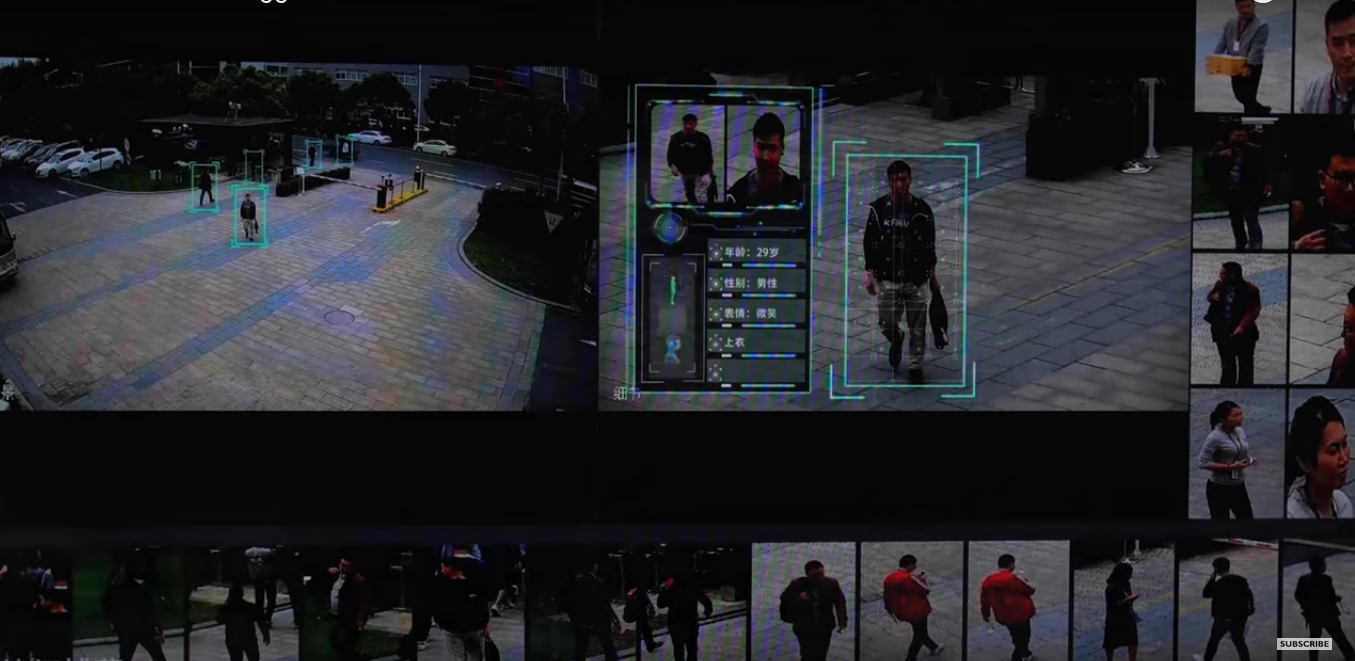
\includegraphics[width=0.8\textwidth]{1_01.png}
%\caption{Những nhà quản lý cho rằng hệ thống có khả năng so khớp khuôn mặt với chứng từ, ước lượng tuổi, dân tộc, giới tính}
%\end{figure}


\begin{figure}[h] \label{fig:three-alternative-operations}
	\centering
	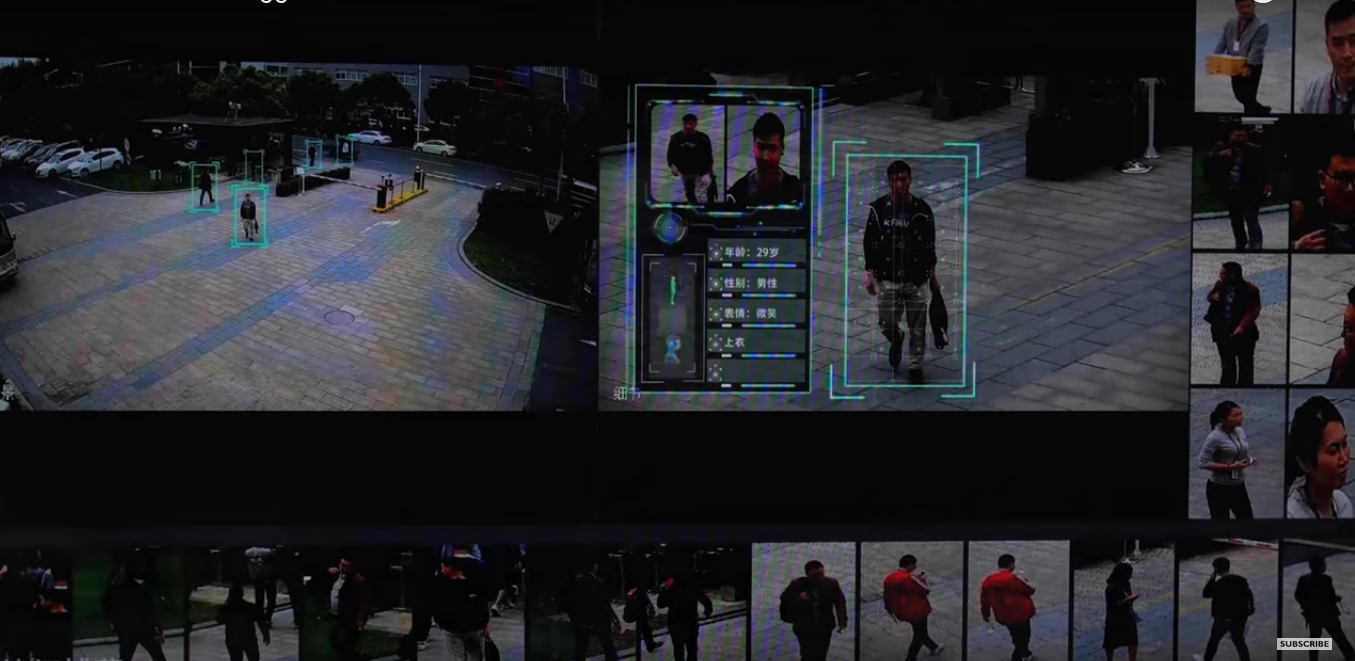
\includegraphics[width=0.9\textwidth]{1_01.png}\\
	Hình a\\
	\color{black}
	%\captionsetup{width=.8\textwidth}
	\begin{tabular}{cc}
		\\
		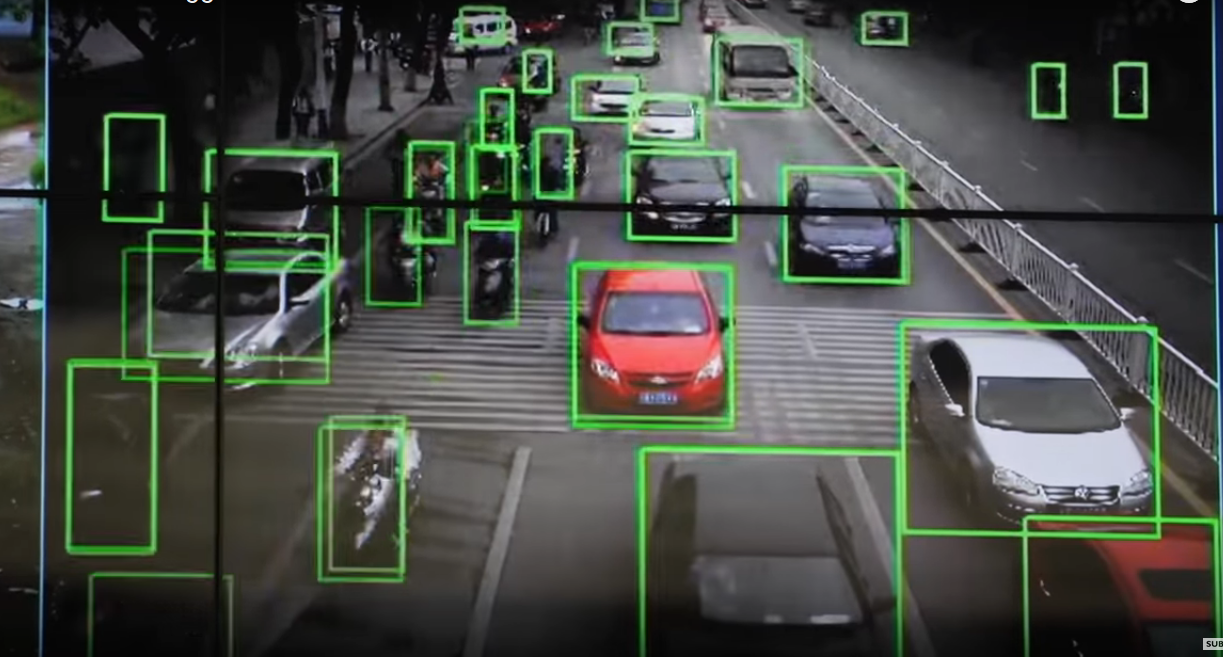
\includegraphics[width=0.5\textwidth]{1_02.png} &
		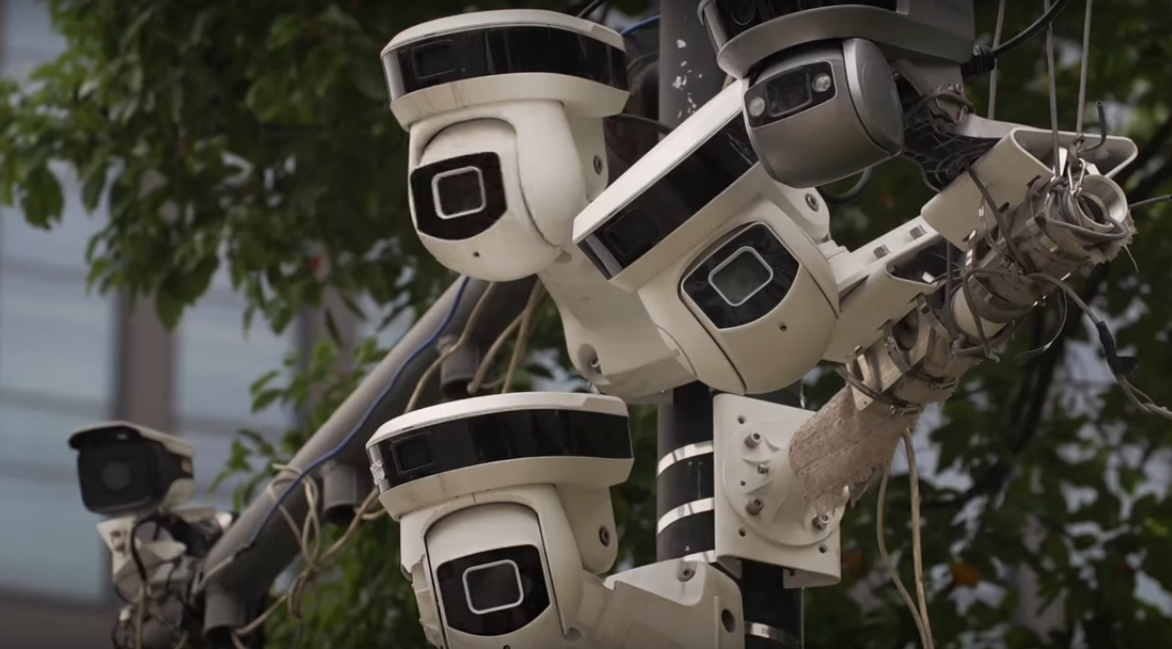
\includegraphics[width=0.49\textwidth]{1_03.png} \\
		
		Hình b & Hình c
	\end{tabular}

	\caption{Hệ thống giám sát video được trải khai tại Trung Quốc} Nhà quản lý của hệ thống này cho rằng có khả năng so khớp khuôn mặt với
	chứng từ cá nhân, dự đoán tuổi, giới tính và dân tộc (Hình a). Hệ thống còn có khả năng theo dõi xe hơi của người dân qua biển số (Hình b). 
	Một vị trí được gắn camera tích hợp trí tuệ nhân tạo dày đặc (Hình c) 
	\footnote{ Hình ảnh được trích xuất từ video https://www.bbc.com/news/av/world-asia-china-42248056/in-your-face-china-s-all-seeing-state}
\end{figure}	
\footnotetext[1]{avc}
\section{Tính thực tiễn}
Một số vấn đề thực tế và khả năng ứng dụng của đề tài: \footnote[3]{text}
\begin{itemize}
\item Phát hiện ngủ gật. Hằng năm ở nước ta vẫn tồn tại những vụ tai nạn thương tâm xảy 
ra do tài xế ngủ gật, khi tìm kiếm với từ khóa "tai nạn do ngủ gậc" Google trả về  gần 3 triệu kết 
quả trong hơn nửa giây hay số lượng lớn bài báo liên quan tới ngủ gậc khi tìm kiếm trên 
báo trực tuyến tuoitre.vn (Hình \ref{drowsiness}.a) . Một hệ thống phát hiện trạng thái của lái xe có thể giảm thiểu khả 
năng xảy tai nạn thảm khốc hằng năm. Một hệ thống được lắp đặt trên xe và đủ thông minh 
để xử lí các tình huống khác nhau ở trong các điều kiện khác nhau trong thực tế. 

\item Tìm kiếm nội dung trong video. Ứng dụng này liên quan tới việc giải các bài toán 
phân loại (classification), phát hiện đối tượng (object detection), theo vết (tracking) hay đếm (counting).
Giả sử có thể xây dựng một hệ thống giám sát trong các trung tâm thương mại, các khu chung cư lớn, 
có khả năng theo dõi đặc điểm của con người như giới tính, các phụ kiện thời trang đi kèm như túi xách, balo, ..,
có đeo kính mắt, có đội mũ hay không? Ứng dụng đầy hứa hẹn khi tìm kiếm người có đặc điểm được mô tả 
hay, tìm kiếm những đứa trẻ đi lạc trong trung tâm thương mại, hay cảnh báo an ninh cho các tổ chức tài
chính, ngân hàng. 

\item Giám sát giao thông. 
\footnotetext[1]{Hình ảnh từ http://tuoitre.vn}
\footnotetext[2]{Hình ảnh từ https://thenextweb.com/artificial-intelligence/2018/03/23/affectivas-automotive-ai-could-keep-distracted-and-drowsy-drivers-from-causing-accidents/}
\end{itemize}

\begin{figure}[h] 
	\centering
	\color{black}
	%\captionsetup{width=.8\textwidth}
	\begin{tabular}{cc}
		\\
		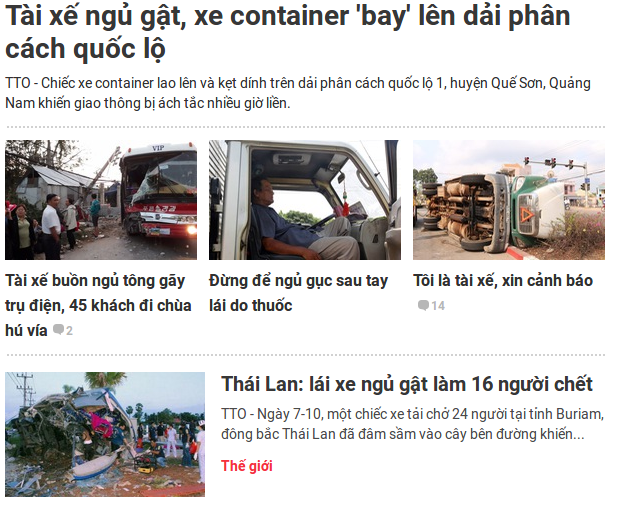
\includegraphics[width=0.5\textwidth]{1_04.png} &
		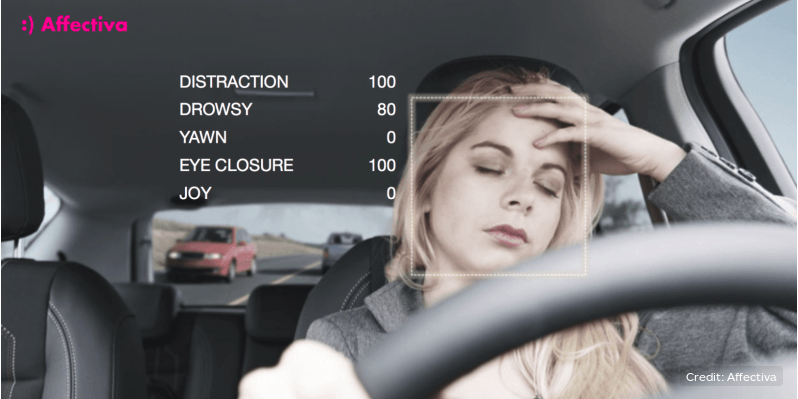
\includegraphics[width=0.49\textwidth]{1_06.png} \\
		
		Hình a \footnote[1]{Hình ảnh từ http://tuoitre.vn} & 
		Hình b \footnote[2]{Hình ảnh từ https://thenextweb.com/artificial-intelligence/2018/03/23/affectivas-automotive-ai-could-keep-distracted-and-drowsy-drivers-from-causing-accidents/}
	\end{tabular}

	\caption{Tình trạng ngủ gậc \& Mô phỏng hệ thống phát hiện ngủ gậc}
	\label{drowsiness}
\end{figure}	

%------------- example of video surveilances ---------------------------------
\begin{figure}[h!]
\centering
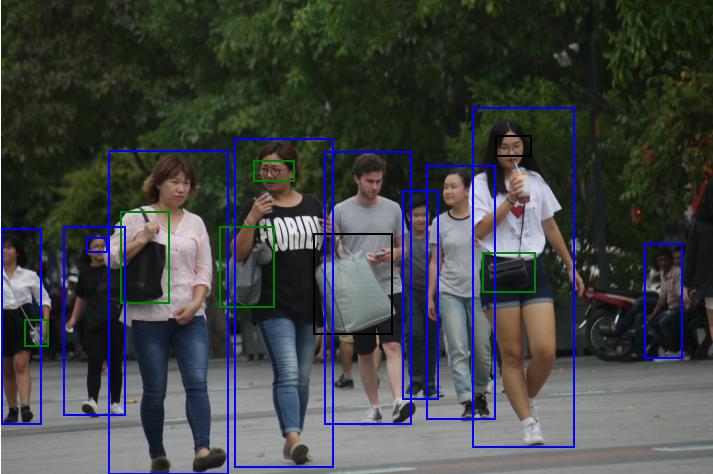
\includegraphics[width=0.8\textwidth]{1_05.png}
\caption{Một ví dụ về giám sát, nhận dạng đặc điểm con người}
\end{figure}

\section{Mục tiêu của luận văn}
Hai nhiệm vụ của luận văn được đặc ra bao gồm:
\begin{itemize}
\item Thử nghiệm và tìm cách cải tiến mô hình SSD, khắc phục nhược điểm của mô hình SSD là khả năng phát hiện đối tượng có kích thước nhỏ.
\item Triển khai hệ thống đã thử nghiệm lên board Jetson TX2.
\end{itemize} 

\section{Quy trình thực hiện luận văn}
Quá trình thực hiện đề tài gồm các bước chính sau: 
\begin{itemize}
	\item  Bước 1: Tìm hiểu và phân tích đề tài, đưa ra các vấn đề chính cần giải quyết
	\item  Bước 2: Nghiên cứu, tìm hiểu các phương pháp, thuật toán có thể áp dụng vào đề tài.
	\item  Bước 3: Tìm kiếm các tập dữ liệu có sẵn và tự xây dựng tập dữ liệu mới, chỉnh sửa và rút trích những thông tin cần thiết để sử dụng cho quá trình huấn luyện và kiểm thử. 
	\item  Bước 4: Thực hiện kiểm thử và đưa ra đánh giá, lặp lại bước 2
	\item  Bước 5: Đề xuất phương pháp cải tiến, hiện thực và đánh giá ưu điểm, nhược điểm của phương pháp.
\end{itemize} 

\chapter{KIẾN THỨC NỀN TẢNG}
Chương này sẽ tập trung trình bày các kiến thức nền tảng, quá trình phát triển của bài 
toán phát hiện đối tượng, ưu điểm của giải pháp deep learning so với phương pháp thị giác 
máy tính truyền thống. Đồng thời chương này cũng cung cấp những cơ hội và thách thức mà 
điện toán cạnh mạng mang lại. 

\section{Kiến thức xử lý ảnh}
\subsection{Bài toán phát hiện đối tượng}
Về cơ bản, một hệ thống Phát hiện đối tượng sẽ nhận đầu vào là một bức ảnh chưa qua xử lý, 
và đầu ra là kết quả các box biên bao quanh đối tượng và xác suất phân loại đối tượng đó 
thuộc lớp nào. Như đã trình bày ở phần giới thiệu, bài toán phát hiện đối tượng là sự kết
hợp hai bài toán định vị đối tượng (localization) bằng cách vẽ các box biên thích hợp bao 
quanh đối tượng sau đó thực hiện phân loại (classification) các đối tượng này. Điều này đòi 
hỏi hệ thống thực hiện tác vụ phức tạp hơn so với các hệ thống truyền thống chỉ thực hiện
chức năng phân loại ảnh. 

\subsection{Phương pháp thị giác máy tính truyền thống}
Nhiều năm về trước, bài toán object detection thường sử dụng những thuật toán đơn giản, tốc độ tính toán nhanh, nhưng bù lại độ chính xác không tốt như sử dụng deep learning.
\subsubsection*{Trích xuất thuộc tính}
Trích xuất thuộc tính(feature extraction) là một quá trình nhằm biến dữ liệu phức tạp đầu vào thành một cách biểu diễn dữ liệu đơn giản hơn, phù hợp hơn cho các thuật toán học máy. Dữ liệu sau khi xử lý đã được lược bỏ phần dữ liệu dư thừa, giữ lại những dữ liệu có ích cho bài toán cần xử lý.
\\

Trong bài toán object detection, đầu vào của dữ liệu là hình ảnh , vì thế để đơn giản hơn cho việc tính toán chúng ra sử dụng một số thuật toán để trích xuất như HOG, SIFT. Trong nội dung bài viết này, tôi không đi sâu về các thuật toán trích xuất dữ liệu này.

\subsubsection{HOG}
Histogram of Oriented Gradients(HOG) là một thuật toán để trích xuất thuộc tính hình ảnh.
Histogram of Oriented Gradient ban đầu được thiết kế ddeer được phát hiện người trong anh nhưng sau đó được mở rộng ra cho các bài toán phát hiện đối tượng. Phương pháp này dựa trên việc đếm số lần xuất hiện các hướng đạo hàm trong ảnh.
\\

Bản chất của phương pháp HOG là thông tin về hình dáng và vẻ bề ngoài đối tượng trong ảnh được mô tả bằng sự phân bố các cường độ gradient hoặc các hướng biên. Mỗi bức ảnh được chia nhỏ thành các phần nhỏ hơn gọi là “tế bào” (cells). Mỗi “tế bào” sẽ ứng với một histogram về các hướng gradient được tính cho các điểm (pixel) nằm trong “tế bào”. Ghép các histogram với nhau ta sẽ có một biểu diễn cho bức ảnh ban đầu. Để tăng cường hiện năng nhận dạng, các histogram ứng với các “tế bào” có thể được chuẩn hóa về độ tương phản bằng các tính một ngưỡng cường độ trong một khối (block) bao gồm các “tế bào” và sử dụng giá trị ngưỡng đó để chuẩn hóa tất cả các “tế bào” trong khối đó. Kết quả của bước chuẩn hóa này là vector đặc trưng có tính bất biến cao hơn đối với các thay đổi về điều kiện ánh sáng.

\begin{figure}[h!]
	\centering
	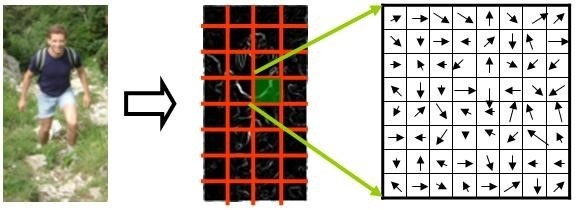
\includegraphics[width=0.8\textwidth]{2_hog.png}
	\caption{Hình ảnh minh họa về HOG}
\end{figure}

Để phát hiện đối tượng với HOG ta tiến hành các bước sau:
\begin{enumerate}
\item Bước 1: Chuẩn bị P mẫu ảnh có chứa đối tượng cần phát hiện và trích xuất các vector đặc trưng HOG từ các mẫu này
\item Bước 2: Chuẩn bị N mẫu không chứa đối tượng cần phần hiện (N>>P) và trích xuất ra vector đặc trưng HOG.
\item Bước 3: Sử dụng bộ phân loại SVM (Support Vector Machine) tuyến tính để học với vector được trích xuất từ bước 1 và bước 2
\item Bước 4: Đối với mỗi bức ảnh trong N mẫu, sử dụng một cửa sổ trượt (sliding window) di chuyển qua tất các vị trí của ảnh. Tại mỗi vị trí thực hiện tính HOG của cửa số và đưa vào bộ phân lớp tại bước 3. Nếu bộ phân lớp phân lớp sai thì lưu lại vector tương ứng cùng với xác suất.
\item Bước 5: Lấy các vector phân lớp sai và sắp xếp theo xác suất nhận dạng cho vào bộ phân lớp để học lại.
\item Bước 6: Áp dụng bộ phân lớp đã được học với các ảnh cần phát hiện.
\end{enumerate}


\begin{figure}[h!]
	\centering
	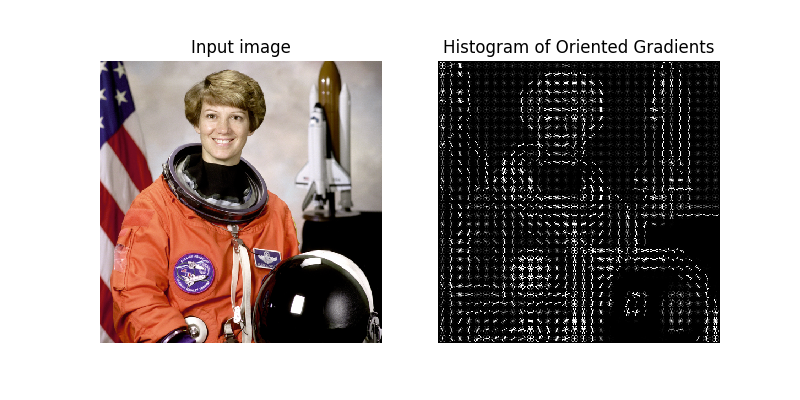
\includegraphics[width=0.8\textwidth]{2_hog_.png}
	\caption[Một ví dụ về đầu ra của HOG]{Trích xuất thuộc tính bằng HOG bảo toàn thông tin về đường viền của đối tượng trong ảnh, làm mất đi các thông tin về màu sắc, giảm độ sắc nét của dữ liệu. }
\end{figure}

Giải quyết bài toán object detection bằng các phương pháp cổ điển có ưu điểm là cần năng lực tính toán thấp, mô hình đơn giản, tốc độ xử lý nhanh. Nhưng trong quá trình xử lý làm mất đi nhiều thông tin giá trị của hình ảnh như màu sắc, độ sắc nét. Dẫn tới độ chính xác không cao.

\subsection{Phương pháp học sâu}
\subsubsection{R-CNN}
R-CNN là tiền thân của mạng Faster R-CNN. \\

R-CNN (Region-based Convolutional Neural Network, 2014), gồm 3 bước:
\begin{enumerate}
    \item Dùng giải thuật Selective Search quét ảnh đầu vào các vùng có thể chứa đối tượng. (generating ~2000 region proposals)
    \item Cho các vùng dự đoán qua một mạng CNN
	\item Lấy đầu ra của các CNN ở bước 2:
	\begin{enumerate}
        \item Làm đầu vào của một bài toán phân loại SVM
        \item Làm đầu vào của một linear regressor to tighten the bb of the object, if such an object exists.
	\end{enumerate}
\end{enumerate}

Một mạng R-CNN được mô tả như hình.
%------------- example of video surveilances ---------------------------------
\begin{figure}[h!]
	\centering
	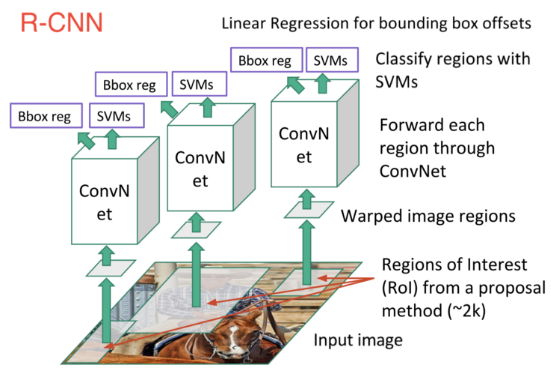
\includegraphics[width=0.7\textwidth]{2_rcnn.png}
	\caption{Mô phỏng một mạng R-CNN \cite{detectionoverview}}
	\end{figure}

Đầu tiên, dự đoán các vùng có thể chứa object (propose regions), trích xuất các đặc trưng
và phân loại các vùng dự đoán dựa trên các đặc trưng của chúng. Về bản chất, bài toán thực
chất là bài toán phân loại truyền thống. R-CNN rất trực quan nhưng rất chậm và kết quả 
không tối ưu. (Chậm vì phải chạy thuật toán Selective Search, mỗi propose regions phải 
qua một lớp CNN, SVMs khá phức tạp với bài toán phân loại n lớp. Do quá trình propose 
regions và trích xuất đặc trưng tách biệt với nhau, nên kết quả học không được tối ưu, 
điều này sẽ được giải thích kỹ hơn ở các mô hình tiếp theo).

\subsubsection{Fast R-CNN}
Fast R-CNN cải thiện tốc độ của R-CNN bằng hai thay đổi chính:

\begin{enumerate}
	\item Thực hiện trích xuất đặc trưng trên bức ảnh trước khi dự đoán vùng chứa đối tượng, 
do đó nó chỉ cần một bước CNN cho toàn bộ bức ảnh thay vì hơn 2000 bước CNN tương ứng với 2000 vùng dự đoán như R-CNN.
	\item  Thay thế SVM bằng lớp softmax. Thực chất SVM là một mô hình phân loại n class, 
với softmax chỉ cần thêm vào mô hình hiện tại thay vì tạo một mô hình phân loại như SVM.   
\end{enumerate}

%------------- example of fast rcnn---------------------------------
\begin{figure}[h!]
	\centering
	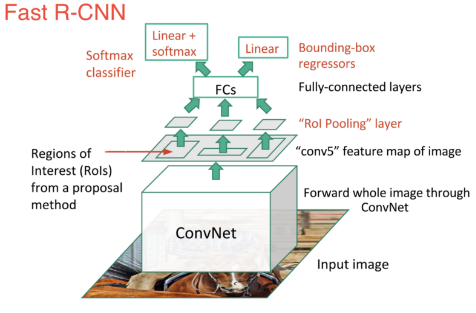
\includegraphics[width=0.7\textwidth]{2_fast.png}
	\caption{Mô phỏng một mạng Fast R-CNN \cite{detectionoverview}}
\end{figure}

Như hình minh họa, các vùng được dự đoán chứa các đối tượng sẽ được sinh ra dựa vào 
feature map cuối cùng của lớp CNN, không phải từ ảnh gốc như R-CNN. Kết quả là chỉ cần 
uấn luyện một lớp CNN cho toàn bộ bức ảnh. \\

Một điểm khác biệt khác, thay vì huấn luyện một mô hình phân loại SVM cồng kềnh thì 
việc sử dụng một lớp softmax giúp tính toán ra trực tiếp xác suất phân loại của mỗi lớp. 
Lúc này, chỉ cần phải huấn luyện một mạng CNN thay vì nhiều mạng CNN và mô hình phân loại 
SVM. \\

Fast R-CNN đã khắc phục được nhược điểm về tốc độ của R-CNN. Nhưng vẫn còn tồn tại một
 "nút thắt cổ chai" trong Fast R-CNN đó là thuật toán selective search phát hiện các 
 vùng dự đoán. 

\subsubsection{Faster R-CNN}
%\subsubsection{FCN}
Faster R-CNN hướng đến việc giải quyết yếu điểm của Fast R-CNN là giải thuật selective
 search. Faster R-CNN thay giải thuật selective search bằng một mạng RPN (Region Proposal
 Network).\\

 %%% sliding window %%%%
\begin{wrapfigure}{r}[0pt]{0.5\linewidth}
	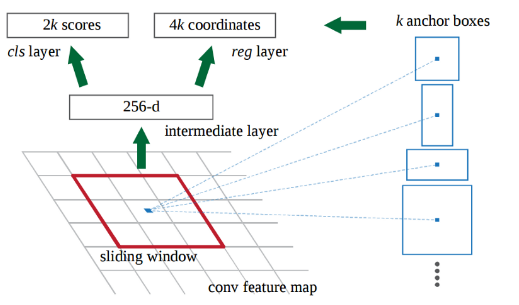
\includegraphics[scale=0.45]{2_slide.png}
	\caption{caption thôi \cite{detectionoverview}}
\end{wrapfigure}

RPN thực hiện như sau:
\begin{itemize}
\item Tại lớp cuối cùng của CNN ban đầu, dịch chuyển một cửa sổ trượt có kích thước 3x3 
trên toàn bộ feature map và ánh xạ vào một lớp có kích thước nhỏ hơn. (256-d)
\item Tại mỗi vị trí trên feature map, nó sinh ra  k vùng dự đoán hay các anchor boxes (default bouding box)
\item Mỗi vùng dự đoán bao gồm: điểm của đối tượng (objectness score - tỉ lệ xuất hiện của đối tượng trong bounding box) cho vùng đó và 4 tham số cx, cy, w, h biểu diễn cho bounding box.
\end{itemize}

Nói cách khác, tại mỗi vị trí (location) trong feature map cuối cùng, xét k bounding box 
có hình dạng khác nhau: box cao, dài, rộng, vuông, ...Mỗi box có 5 tham số, 4 tham số thể 
hiện tọa độ của bounding box, tham số còn lại thể hiện trong bounding box có chứa đối 
tượng hay không.\\

\begin{figure}[h!]
	\centering
	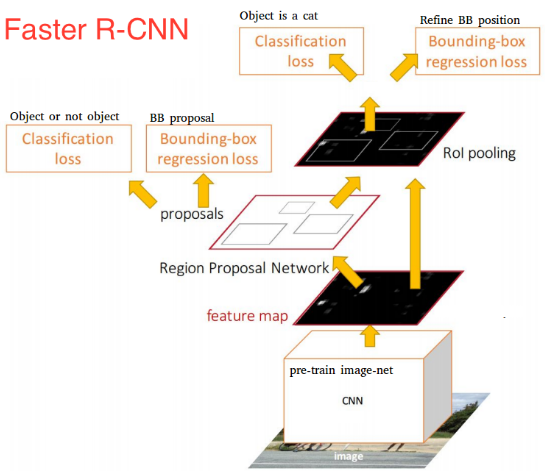
\includegraphics[width=0.7\textwidth]{2_faster.png}
	\caption[Caption for LOF]{Mô phỏng một mạng Faster R-CNN \cite{detectionoverview}} 
\end{figure}

Trong hình (), 2k score thể hiện xác suất bounding box chứa đối tượng của k bounding box.
Lưu ý rằng RPN chỉ xuất ra tọa độ của bounding box, vai trò của nó vẫn là đưa ra các vùng 
dự đoán (propose regions), chứ không cố gắng thực hiện phân loại các đối tượng nằm trong 
vùng đó. Nếu anchor box có tỉ lệ xuất hiện đối tượng (objectness score) lớn hơn một ngưỡng 
nào đó, thì tọa độ anchor box đó là sẽ là vùng dự đoán cần tìm (region proposal). \\
 
Khi đã có tìm được các vùng dự đoán, đó chính là đầu vào của mạng Fast R-CNN. Từ mạng 
Fast R-CNN, thêm vào các lớp pooling, các lớp fully-connected, và cuối cùng là lớp softmax
 và bounding box regressor. Tóm lại, Faster R-CNN = RPN + Fast R-CNN.\\

 
Faster R-CNN nhanh hơn và chính xác hơn so với Fast R-CNN hay trước đó là R-CNN
 nhưng đều sử dụng một triết lý thiết kế chung, đó là sinh ra các vùng dự đoán 
 trước, sau đó thực hiện phân loại các vùng dự đoán này. Nhưng so với các mạng 
 ra đời sau, Faster R-CNN vẫn còn phức tạp và chưa đáp ứng được yêu cầu về thời gian thực. 

\subsection{Một số mô hình xử lý hợp nhất}
\subsubsection{SSD}
Single Shot Detector, có tốc độ gấp nhiều lần Faster R-CNN. \\

Các mô hình ở trên đều thực hiện dự đoán vùng chứa đối tượng và phân loại các 
vùng dự đoán này theo hai bước hoàn toàn độc lập. SSD thực hiện cả hai bước trong
cùng một mạng, thực hiện đồng thời việc dự đoán bounding box và phân loại class,
 do đó gọi là "single shot".\\

Cụ thể, đầu vào là một bức ảnh cùng với một tập các grouth truth box được gắn labels, SSD làm như sau:
\begin{enumerate}
	\item Đưa ảnh đầu vào qua một loạt các lớp tích chập, thu được một tập các feature map có kích thước khác nhau (eg 38x38, 19x19, 9x9, ..)
	\item Tại mỗi vị trí trên feature map này, sử dụng các bộ lọc 3x3 để đánh giá một nhóm các default bounding box. Các default bounding box này tương đương với anchor box trong mạng Faster R-CNN.`
	\item Với mỗi box, đồng thời dự đoán bounding box offset và xác suất phân loại. 
	\item Trong suốt quá trình huấn luyện, bổ sung
\end{enumerate}

\subsection{Một số mô hình phân loại}
Vì các mô hình phân loại được sử dụng làm mạng nền của các mô hình phát hiện, nó ảnh hưởng trực tiếp đến kết quả cũng như tốc độ của mô hình phát hiện. Vì vậy việc thiết kế và sử dụng mô hình phân loại thích hợp là hết sức quan trọng. \\


\section{Edge Computing}
\subsection{Cloud computing}	
	Trong những năm gần đây, điện toán đám mây (Cloud computing) được sử dụng trong nhiều lĩnh vực, tạo nên một cuộc cách mạng trong ngành công nghiệp công nghệ thông tin, thay đổi thói quen lưu trữ, sử dụng tài nguyên máy tính của nhiều doanh nghiệp. Các nền tảng điện toán đám mây phổ biến, đươc nhiều doanh nghiệp sử dụng có thể kể đến như Amazon Web Service (AWS), Microsoft Azure Cloud Computing.Về bản chất, Cloud Computing là mô hình điện toán mà việc sử dụng tài nguyên máy tính thông qua internet. Mô hình điện toán này tập trung các máy tính và cung cấp dịch vụ trên internet theo nhu cầu của người sử dụng. Nhờ sức mạnh của điện toán đám mây mà người sử dụng không phải sử dụng máy tính của họ để thực thi các tác vụ nặng, tốn nhiều thời gian. Họ chỉ cần thuê một dịch vụ điện toán đám mây, thông qua internet để truy cập vào các cloud sau đó tận dụng sức mạnh trên cloud để chạy các ứng dụng cần thiết. 	\\
	
%-------------2_111 Ví dụ CNN convolution-----
\begin{figure}[h]
\centering
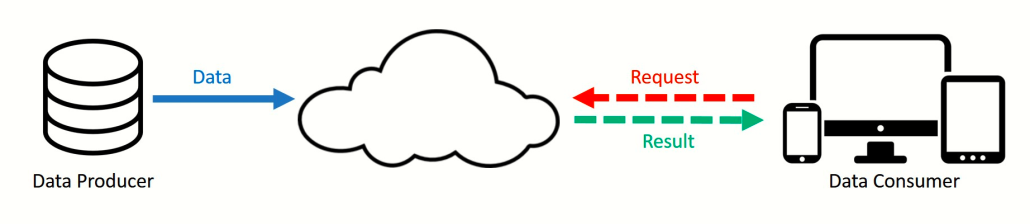
\includegraphics[width=0.9\textwidth]{cloud.png}
\caption{\label{fig:2.3333}   Mô hình cloud computing}
\end{figure}
% ---------------------------------


	Nhờ có điện toán đám mây mà doanh nghiệp có thể linh động trong việc sử dụng tài nguyên. Chỉ cần gửi request thì nhà cung cấp dịch vụ sẽ tự tìm kiếm tài nguyên để thực thi.  Dựa vào đó, doanh nghiệp sẽ tiết kiệm được chi phí đầu tư cho việc xây dựng, bảo trì và mở rộng hệ thống máy chủ của mình. Hơn nữa, việc chạy ứng dụng sẽ do bên nhà cung cấp dịch vụ hỗ trợ nên doanh nghiệp sẽ ko phải thuê nhân viên IT để vận hành ứng dụng. Có thể nói điện toán đám mây đã tạo điều kiện cho các doanh nghiệp hoạt động hiệu quả và tiết kiệm chi phí hơn, đặc biệt là các doanh nghiệp vừa và nhỏ khi không phải tốn một khoản chi phí đầu tư ban đầu lớn.
\subsection{Edge computing}
Cloud Computing là một cuộc cách mạng lơn đối với ngành công nghiệp máy tính. Tuy nhiên, với sự phát triển các thiết bị cảm biến và di đông, Internet of Things (IoT) ngày càng phổ biến trong các lĩnh vực đời sống. Do vậy, lượng dữ liệu sinh ra hằng ngày cực kì khủng lồ. Theo như dự đoán của Cisco Global Cloud Index, đến năm 2019, lượng dữ liệu sinh ra bởi con người, máy móc sẽ lên đến 500 zettabytes, tuy nhiên các trung tâm dữ liệu chỉ đáp ứng được 10.4 zettabytes. Vì mấy chúng ta cần một mô hình để giải quyết dữ liệu trước khi được đưa lên cloud, gọi là Edge Computing.

\subsubsection{Tại sao chúng ta cần sử dụng Edge Computing?} 

Đầu tiên, việc thực thi các tác vụ trên cloud đã chứng minh đươc hiệu quả trong việc xử lí dữ liệu bởi vì sức mạnh tính toán trên cloud vượt trội so với việc tính toán ở cạnh (edge). Tuy nhiên, so với tốc độ phát triển nhanh chóng của xử lí dữ liệu, thì hạ tầng mạng vẫn chưa đáp ứng được. Tốc độ truyền nhận dữ liệu trở thành nút nghẽn cổ chai nếu chúng ta chỉ sử dụng một mô hình Cloud Computing. Ví dụ, xe tự hành sẽ sinh ra 1GB dữ liệu trong vòng 1s và yêu cầu xử lí, đưa ra các quyết định trong thời gian thực (real-time). Nếu toàn bộ dữ liệu được đưa chuyển về cloud tính toán rồi đưa ra quyết định ngược trở lại về xe thì sẽ không đáp ứng được thời gian đáp ứng. Vì vậy cần phải xử lí các dữ liệu và đưa ra quyêt định ngay trên xe (edge) và chỉ chuyển những thông tin về vị trí, tốc độ về cloud.
Tiếp theo, các thiết bị điện tử trong mô hình IoT vừa đóng vai trò sử dụng dữ liệu từ cloud, vừa sinh ra dữ liệu. Tuy nhiên, các dữ liệu này chỉ ở dạng thô (raw data), hơn nữa các thiết bị được sản xuất bởi nhiều nguồn khác nhau nên việc chuẩn hóa dữ liệu cực kì khó khăn, vì vậy việc xử lí dữ liệu này tại cloud không thật sự hiệu quả. Điều này có nghĩa là phần lớn dữ liệu sẽ không được chuyển về cloud, mà sẽ có một bước xử lí trung gian tại cạnh. Cuối cùng là về vấn đề năng lương, các thiết bị IoT tiêu thụ cực kì ít năng lượng, vì vậy sử dụng mạng không dây để truyền nhận một lượng dữ liệu lớn như vậy sẽ khiến cho nguồn năng lượng không đảm bảo.

\subsubsection{Edge computing là gì}
Edge computing là mà một mô hình cho phép công việc tính toán được tiến hành ngay tại cạnh của network, chỉ gửi những dữ liệu đã xử lí về về cloud. Có nghĩa là việc tính toán sẽ diễn ra gần hoặc tại nguồn dữ liệu.

%-------------2_111 Ví dụ CNN convolution-----
\begin{figure}[h]
\centering
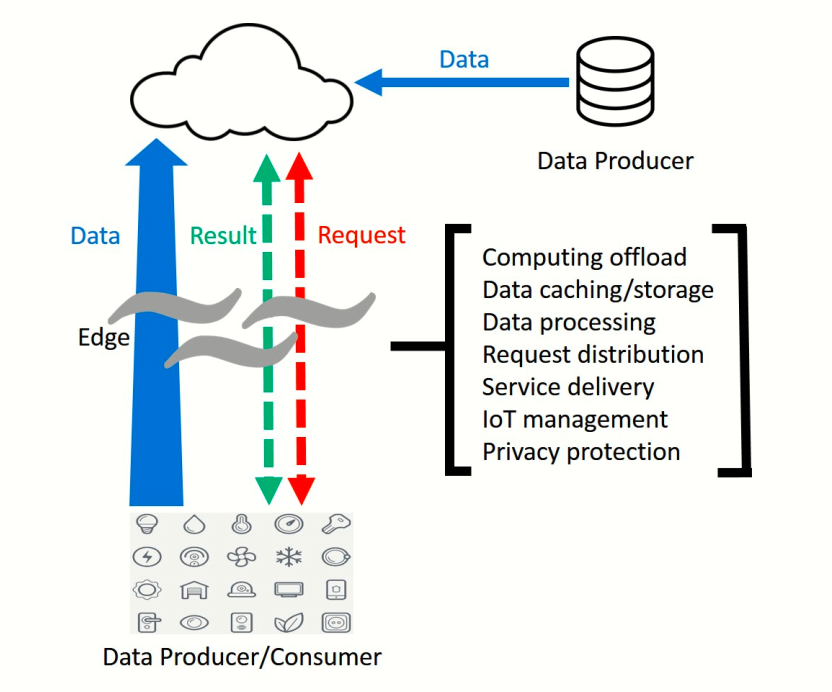
\includegraphics[width=0.7\textwidth]{edge.png}
\caption{\label{fig:2.444}  Mô hình Edge Computing}
\end{figure}
% ---------------------------------
	
\subsubsection{Ứng dụng của Edge Computing}
\begin{itemize}
\item \textbf{Xử lý video}:\\

Sự phổ biến của các thiết bị di động và mạng lưới camera làm cho nhu cầu xử lý và phân tích video ngày một tăng cao. Cloud Computing không còn phù hợp với các ứng dụng phân tích video bởi vì tốn chi phi truyền tải, độ trễ và vấn đề bảo mật. Ngày nay, camera được lắp dặt rộng rãi trên toàn thành phộ và trên các phương tiện giao thông. Khi một đứa trẻ bị lạc, thì có khả năng hình ảnh của đứa trẻ sẽ được ghi lại bởi bất kì camera nào. Tuy nhiên, dữ liệu từ camera thường không được tải lên cloud bởi vì vấn đề cá nhân và chi phí đường truyền. Điều này khiến cho công việc tìm kiếm trở nên rất khó khăn. Ngay cả khi data được tải lên cloud, thì với lượng lớn dữ liệu thì việc tìm kiếm rất mất thời gian. Với edge computing, một yêu cầu tìm kiếm được gửi từ cloud đến tất cả các thiết bị trong khu vực. Các thiết bị không cần phải tải toàn bộ data, mà chỉ cần thông báo kết quả có hay không. Nhờ vào đó, ta tận dụng được sức mạnh tính toán từ tất cả thiết bị và có kết quả nhanh hơn.

\item \textbf{Smart city}:\\

Edge Computing có thể được sử dụng từ một ngôi nhà đến khu vực và ngay cả toàn bộ một thành phố.  Việc tính toán diễn ra càng gần nguồn dữ liệu càng tốt. Với mô hình này, một yêu cầu được gửi từ server và sẽ được xử lí tại các cạnh của mạng. Edge Computing là một mô hình lý tưởng cho Smart City:
Lượng dữ liệu lớn: một thành phố dân số một triệu dân có thể sinh ra lượng dữ liệu 180PB/ngày từ phương tiện giao thông, thiết bị y tế, …. Xây dựng một trung tâm dữ liệu để xử lí lượng dữ liệu đó gần như bất khả thi. Trong trường hợp này, Edge Computing là một giải pháp hiêu quả để tiền xử lí dữ liệu.\\

Độ trễ thấp: Nhiều ứng dụng yêu cầu khả năng dự đoán chính xác và nhanh chóng. Edge Computing có thể giảm thiếu tối đa độ trễ so với việc tập trung và xử lí dữ liệu tại cloud.
\end{itemize}

\subsubsection{Thách thức và cơ hội}
Để hiện thực và triển khai mô hình Edge Computing, chúng ta cần kết hợp cả hệ thống tính toán và hạ tầng mạng. Điều đó mang đến nhiều thách thức bao gồm khả năng lập trình (programmability), naming, quảng lí dịch vụ, chính sách bảo mật, riêng tư và tối ưu hóa.
\begin{itemize}
\item \textbf{Programmability}:\\

Đối với Cloud Computing, người dùng lập trình và triển khai ngay trên cloud. Nhà cung cấp dịch vụ chịu trách nhiệm về tài nguyên tính toán. Tuy nhiên đối với Edge Computing, việc tính toán được đẩy về tại cạnh, và các thiết bị thì thường không thống nhất một nền tảng(platform). Người lập trình phải đối mặt khó khăn để viêt ứng dụng và triển khai các ứng dụng.

\item \textbf{Naming}:\\

Một vấn đề trong Edge là số lượng thiết bị rất lớn. Tương tự như trong các hệ thống máy tính, naming rất quan trọng đối với việc lập trình, định danh và truyền tải dữ liệu. Tuy nhiên, vẫn chưa có bất kì chuẩn hóa nào cho việc định danh trong Edge Computing bởi vì số lượng lớn các thiết bị và rất nhiều giao thức mạng được sử dụng. Một mô hình đặt tên cần đảm bảo tính bảo mật và cá nhân, tính linh động và khả năng mở rộng trong tương lai.


\item \textbf{Quản lí các dịch vụ}:\\

Để sử dụng hiệu quả mô hình Edge Computing, dịch vụ cần phải đáp ứng sự đa dạng, khả năng mở rông, độc lập và độ tin cậy. Với sự phát triển nhanh chóng của IoT, chúng ta mong đợi ngày càng có nhiều dịch vụ được triển khai tại cạnh của mạng. Vì vậy khi xây dựng mô hình mạng cần phải đảm bảo khả năng phát triển và mở rộng thêm các thiết bị. Đó là một thách thức lớn bởi sự đa dạng của các thiết bị. Một vấn đề khác khi xây dựng mô hình là tính độc lập. Khi một thiết bị trong mạng xảy ra sự cố, thì các thiêt bị các cần phải đảm bảo hoạt động bình thường. Cuối cùng là độ tin cậy, chúng ta rất khó để xác định nguyên nhân một dịch vụ hay thiết bị hoạt động không chính xác. Việc bảo trì và nâng cấp mô hình mạng là việc cần thiết để đảm bảo dữ liệu được tính toán và truyền nhận chính xác.

\item \textbf{Tối ưu hóa}:\\

Trong Edge Computing, chúng ta có nhiều lớp với các khả năng tính toán khác nhau. Chúng ta tối ưu hóa chiến lược phân bổ công việc nhằm đảm báo độ trể, băng thông, năng lương và chi phí:\\

\textit{Độ trễ}: là một trong nững tiêu chí đánh giá quan trọng nhất đặc biệt đối với các ứng dụng thời gian thực. \\

\textit{Băng thông}: nâng cấp băng thông đường truyền có thể giảm thời gian truyền tải dữ liệu đặc biệc đối với các dữ liệu lớn như video, hình ảnh. \\

\textit{Năng lượng}:
 là vấn đề tối quan trọng trong đối với các thiết bị trong mạng. Chúng ta phải giải quyết bài toán tối ưu năng lượng sử dụng giữa tính toán tại cạnh và truyền tải dữ liệu.\\
 
\textit{Chi phí}: Tương tự như năng lượng, chúng ta cần cân đối giữa chi phí năng lượng tiêu thụ tại cạnh, đường truyền và chi phí cho các dịch vụ Cloud Computing.
\end{itemize}

\chapter{CÁC CÔNG TRÌNH LIÊN QUAN }
\section{Single Shot MultiBox Detector}
\subsection{Đặc điểm chính của SSD}
Mô hình ssd dựa xây dựng dựa trên một mạng tích chập lan truyền thẳng sinh ra một tập cố định các box dự đoán và điểm tương ứng với khả năng xuất hiện đối tượng trong box dự đoán, theo sau là một bước Non-Maximum suppression để sinh ra kết quả dự đoán cuối cùng. \\

\begin{figure}[h!]
	\centering
	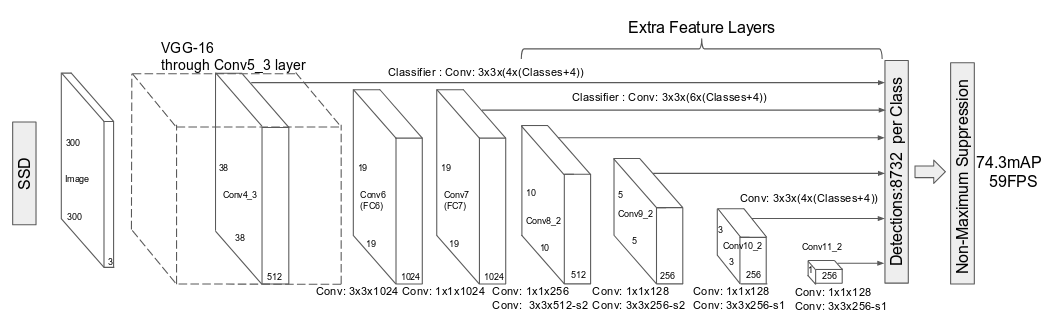
\includegraphics[width=0.9\textwidth]{3_ssd_arch.png}
	\caption[Caption for LOF]{Cấu trúc tổng quát mô hình SSD \cite{ssd}}
\end{figure}

\paragraph*{Sử dụng các bản đồ đặc trưng khác nhau cho dự đoán.} Trong cấu trúc của mạng SSD, qua các lớp tích chập, kích thước bản đồ đặc trưng giảm dần, điều này cho phép thực hiện dự đoán các đối tượng có kích thước đa dạng. Đây là khác biệt lớn nhất giữa SSD và YOLO.\\

\paragraph*{Sử dụng lớp tích chập là lớp dự đoán.} Như đã đề cập ở trên, mỗi bản đồ đặc trưng được lựa chọn vào quá trình dự đoán có thể sinh ra một tập cố định các dự đoán nhờ các bộ lọc tích chập. Ví dụ với bản đồ đặc trưng có kích thước mxn với p kênh,  sẽ sử dụng các bộ lọc có kích thước 3x3xp để có đầu ra là các điểm phân loại đối tượng và tọa độ tương đối của box dự đoán so với box mẫu.\\

\paragraph*{Số lượng box mặc định và tỉ lệ cạnh.} Mỗi ô trên bản đồ đặc trưng được lựa chọn để dự đoán sẽ được liên kết với một tập các box mặc định bằng phép tích chập. Tại mỗi ô trên bản đồ đặc trưng, SSD dự đoán vị trí tương đối của box tiềm năng so với box mặc định và điểm phân loại của mỗi nhãn/lớp mà đối tượng nằm trong box tiềm năng thuộc về. 
Cụ thể, tại một ô trên bản đồ đặc trưng có k box mặc định, chúng ta cần tính toán với bài toán có c nhãn/lớp cần phân loại và 4 tọa độ tương đối so với box mẫu. Kết quả sẽ có (c+4)*k bộ lọc sẽ được áp dụng lên mỗi ô trên bản đồ đặc trưng, tạo ra (c+4)*k*m*n đầu ra cho một bản đồ đặc trưng có kích thước m*n. Hình dưới minh họa    \\

\begin{figure}[h!]
	\centering
	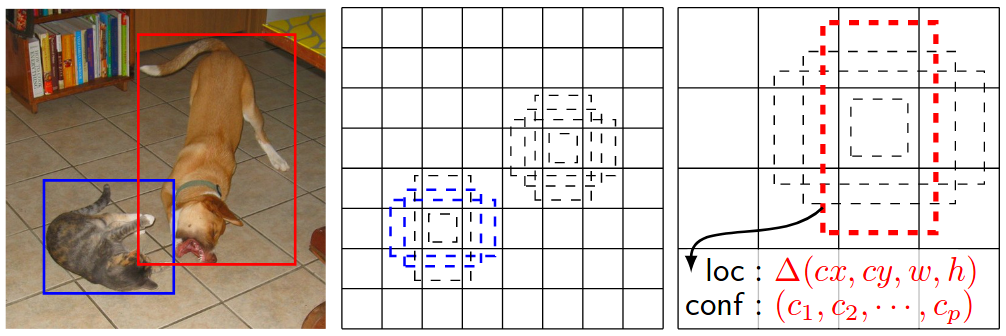
\includegraphics[width=0.9\textwidth]{3_ssd_box.png}
	\caption[Caption for LOF]{box mẫu và box mặc định trong SSD \cite{ssd}}
	Các box mẫu từ ảnh (a) sẽ được gán tương ứng thành các box mặc định ở (b) và (c). Như vậy, thay vì phát hiện các box chứa tuỳ ý, SSD chỉ phát hiện một số box mẫu có tỉ lệ và độ lớn nhất định.  
\end{figure}

\subsection{Cấu trúc mạng SSD}
\begin{itemize}
\item Một framework SSD gồm có 3 phần chính: Base Model, Extra Layers, MultiBox. 
\item Base model có thể sử dụng một số mạng state-of-the-art để trích xuất đặc trưng ảnh như VGG-16, VGG-19, Resnet, AlexNet, GoogLeNet, ... Nhưng trong bản báo cáo này chỉ đề cập đến base model sử dụng mạng VGG-16.
\end{itemize}

\subsubsubsection*{Base Model - VGG-16}
\begin{table}[h]
	\caption{Cấu trúc mạng SSD300 và số lượng tham số của mỗi lớp}
	\begin{tabular}{|l|l|l|}
		\hline
		Layer & Size & Paramters \\
		(windowsize, numfilters, stride, padding) &
		(height, width, channel)& (weights + bias)\\ \hline

		input & [300,300,3] & 0, RF = 1 \\
		& & \\ \hline
		conv\_1\_1 (3, 64, 1, 1) & [300,300,64] & 3x3x3x64 + 64 = 1792\\  
		& & RF=3, j\_out = 1 \\ \hline
		conv\_1\_2 (3, 64, 1, 1) & [300,300,64] & 3x3x64x64 + 64 = 36928 \\
		& & RF=5, j\_out = 1 \\ \hline
		pooling\_1 (2, 0, 2, 0) & [150,150,64] & 0 \\
		&&j\_out=2, RF=7 \\ \hline
		conv\_2\_1 (3, 128, 1, 1) & [150,150,128] & 3x3x64x128 + 128 = 73856\\
		&&j\_out=2, RF=11 \\ \hline
		conv\_2\_2 (3, 128, 1, 1) & [150,150,128] & 3x3x128x128 + 128 = 147584\\
		&&j\_out=2, RF=15 \\ \hline
		pooling\_2 (2, 0, 2, 0) & [75,75,128] & 0\\
		&&j\_out=4, RF=19 \\ \hline
		conv\_3\_1 (3, 256, 1, 1) & [75,75,256] & 3x3x128x256 + 256 = 295168\\
		&&j\_out=4, RF=27 \\ \hline
		conv\_3\_2 (3, 256, 1, 1) & [75,75,256] & 3x3x256x256 + 256 = 590080\\
		&&j\_out=4, RF=35 \\ \hline
		conv\_3\_3 (3, 256, 1, 1) & [75,75,256] & 3x3x256x256 + 256 = 590080\\
		&&j\_out=4, RF=43 \\ \hline
		pooling\_3 (2, 0, 2, 0) (ceil\_mode) & [38,38,256] & 0\\
		&&j\_out=8, RF=51 \\ \hline
		conv\_4\_1 (3, 512, 1, 1) & [38,38,512] & 3x3x256x512 + 512 = 1180160\\
		&&j\_out=8, RF=67 \\ \hline
		conv\_4\_2 (3, 512, 1, 1) & [38,38,512] & 3x3x512x512 + 512 = 2359808\\
		&&j\_out=8, RF=83 \\ \hline
		conv\_4\_3 (3, 512, 1, 1) & [38,38,512] & 3x3x512x512 + 512 = 2359808\\
		&& j\_out=8, RF=99 \\ \hline
		L2Norm & [38, 38, 512] & 0 \\ 
		& & \\ \hline
		pooling\_4 (2, 0, 2, 0) & [19,19,512] &0\\
		&&j\_out=16, RF=115 \\ \hline

\end{tabular}
\end{table}

Giải thích 
\begin{itemize}
	\item đằng sau mỗi convolutional layer đều sử dụng ReLU, có thể sử dụng batch\_norm tùy thuộc vào cách thiết kế, dataset. Các lớp pooling thường sử dụng phép toán max pooling.
	\item L2Norm layer là lớp nhằm chuẩn hóa feature map của lớp conv\ 4\_3. Việc này là để hạn chế overfitting của mô hình.
	\item ceil\_mode: là một paramter trong hàm MaxPool2d() của pytorch. Với mode này thay vì thực hiện max pooling bằng các kernel\_size=[2x2], pytorch sẽ thay thế 1 vài chỗ bằng kernel\_size={[1x1], [1x2], [2x1]}.
	\item dilation: là một kiểu thực hiện phép toán convolution.\\
		 \textbf{Ví dụ}: Một feature map kích thước 7x7, thực hiện phép dilated convolution với dilation = 2.
		 
		 \begin{figure}[h!]
			\centering
			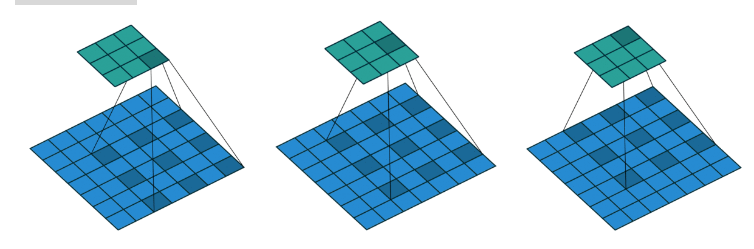
\includegraphics[width=0.9\textwidth]{3_dilation.png}
			\caption[Caption for LOF]{Phép tích chập với dilation = 2 \cite{dilation}}
		\end{figure}

	\item Công thức tính output size của một convolutional layer (height và width, không tính channel) là:\\ 
			\begin{center}
				\begin{tabu}{clc}
					\rowfont{\color{blue}}
					& O = (W-F+2P)/S + 1 & \\
					\\
					Với & O là output size, & \\
						& W là input size. & \\
						& F là kernel size. & \\
						& P là padding. & \\
						& S là stride. & \\

				\end{tabu}
			\end{center}
			Nếu \color{blue} O \color{black} không là số nguyên dương thì phép convolution không hợp lệ.
\end{itemize}

\subsubsubsection*{Extra Layers}
Input của lớp conv\_8\_1 là output của lớp conv\_7.
\begin{table}[h]
	\caption{Cấu trúc mạng chi tiết SSD300 và số lượng tham số của mỗi lớp}
	\begin{tabular}{|l|l|l|}
		\hline
		Layer & Size & Paramters \\
		(windowsize, numfilters, stride, padding) &
		(height, width, channel)& (weights + bias)\\ \hline

		conv\_7 (1, 1024, 1, 0) & [19,19,1024] & 3x3x1024x1024 + 1024 = 9438208 \\
		(thuộc base model) & & \\ \hline
		conv\_8\_1 (1, 256, 1, 0) & [19,19,256] & 3x3x1024x256 + 256 = 2359552 \\ \hline
		conv\_8\_2 (3, 512, 2, 1) & [10,10,512] & 3x3x512x512 + 512 = 2359808 \\ \hline
		conv\_9\_1 (1, 128, 1, 0) & [10,10,128] & 2 \\ \hline
		conv\_9\_2 (3, 256, 2, 1) & [5,5,256] & 3x3x128x256 + 256 = 295168 \\ \hline
		conv\_10\_1 (1, 128, 1, 0) & [5,5,128] & 3x3x256x128 + 128 = 295040 \\ \hline
		conv\_10\_2 (3, 256, 2, 1) & [3,3,256] & 3x3x128x256 + 256 = 295168 \\ \hline
		conv\_11\_1 (1, 128, 1, 0) & [3,3,128] & 3x3x256x128 + 128 = 295040 \\ \hline
		conv\_11\_2 (3, 256, 2, 1) & [1,1,256] & 3x3x128x256 + 256 = 295168 \\ 
		(sử dụng giải thuật astrous) & & \\\hline
\end{tabular}
\end{table}

\subsubsubsection*{MultiBox Layers}
Mỗi output từ các layers sau sẽ được input vào confidence layer và location layer:  
conv\_4\_3, conv\_7, conv\_8\_2, conv\_9\_2, conv\_10\_2, conv\_11\_2. Mỗi pixel 
của các lớp convolutional này sẽ tạo ra 4 hoặc 6 default box. Mỗi default box 
này sẽ được đi qua conf\_conv\_layer và loc\_conv\_layer. \\

\textbf{Ví dụ}: Cụ thể conv\_4\_3 layer sẽ tạo ra 4 boxes (số boxes tạo ra có thể là 6 ở những lớp khác) cho mỗi pixel trong feature map của nó. Mỗi box này sẽ được input vào 2 convolutional layer khác nhau:
\begin{itemize}
\item Loc\_conv\_4\_3 layer sẽ có nhiệm vụ điều chỉnh các bounding box sao cho khớp với ground truth nhất có thể. Lớp này sẽ output ra 4 tham số cho mỗi bounding box được input vào với dạng [cx, cy, width, height]. Với mỗi bounding box, layer này cho ra 4 outputs
\item Conf\_conv\_4\_3 layer có nhiệm vụ xác định vật thể nằm trong bounding box là gì.
Lớp này sẽ trả về xác suất mà bounding box này thuộc từng loại classes, có dạng (c1, c2, ... cn) với c1 là xác suát box có chứ object thuộc loại 1. Với mỗi bounding box, layer sẽ cho ra number\_classes output.
\item Feature map của conv\_4\_3 layer có kích thước là [38x38x512]. Mỗi pixel trong feature map cho ra 4 bounding box. Vậy conv\_4\_3 layer có tổng cộng 4 * 38 * 38 = 5776 bounding boxes.
\end{itemize}

Chi tiết các multi box có thiết lập như sau:

\begin{table}[h]
	\centering
	\caption{Cấu trúc mạng chi tiết SSD300 và số lượng tham số của mỗi lớp}
	\begin{tabular}{|l|l|l|}
		\hline
		Input & Layers & Size \\
		(number of boxes) & (windowsize, numfilters, stride, padding) & \\ \hline
		CONV\_4\_3 & CONF\_CONV\_4\_3 (3, 4*num\_classes, 1, 1)  & [38x38x(4*num\_classes)] \\
		(38x38x4 = 5776) & LOC\_CONV\_4\_3 (3, 4*4, 1, 1) & [38,38,(4*4)] \\ \hline
		CONV\_8\_2 & CONF\_CONV\_8\_2 (3, 6*num\_classes, 1, 1)  & [10,10,(6*num\_classes)] \\
		(10x10x6=600) & LOC\_CONV\_8\_2 (3, 6*4, 1, 1) & [10,10,(6*4)] \\ \hline
		CONV\_9\_2 & CONF\_CONV\_9\_2 (3, 6*num\_classes, 1, 1)  & [5,5,(6*num\_classes)] \\
		(5x5x6=150) & LOC\_CONV\_9\_2 (3, 6*4, 1, 1) & [5,5,(6*4)] \\ \hline
		CONV\_10\_2 & CONF\_CONV\_10\_2 (3, 4*num\_classes, 1, 1) & [3,3,(4*num\_classes)] \\ 
		(3x3x4=36) & LOC\_CONV\_10\_2 (3, 4*4, 1, 1) & [3,3,(4*4)] \\ \hline
		CONV\_11\_2 & CONF\_CONV\_11\_2 (3, 4*num\_classes, 1, 1) & [1,1,(4*num\_classes)] \\
		(1x1x4=4) & LOC\_CONV\_11\_2 (3, 4*num\_classes, 1, 1)  & [1,1,(4*4)] \\ \hline
		Total: 8732 boxes	& & \\ \hline
\end{tabular}
\end{table}

\subsection{Phương pháp huấn luyện }

\subsubsubsection*{Chiến lược chọn box mẫu. \footnotemark[1]{}} Trong quá trình huấn luyện, mô hình cần xác định những box mặc định tương ứng với box mẫu trong dữ liệu huấn luyện để bắt đầu quá trình huấn luyện. Với mỗi box mẫu, mô hình lựa chọn ra các box mặc định có vị trí, tỉ lệ cạnh và kích thước khác nhau thỏa điều kiện tỉ lệ jaccard overlap lớn hơn một ngưỡng, ngưỡng này thường là 0.5. Chiến lược lựa chọn như vậy giúp mô hình tổng quát hơn so với việc chỉ lựa chọn duy nhất một box mặc định tương ứng với một box mẫu được đề cập trong MultiBox. \cite{ssd}
\footnotetext[1]{Nguyên văn: \textit{Matching Strategy}} \\

Mô tả cách tính tỉ lệ jaccard overlap hay tỉ lệ phần giao trên phần hợp IoU \footnote{IoU: Intersection Over Union}
\begin{figure}[h!]
	\centering
	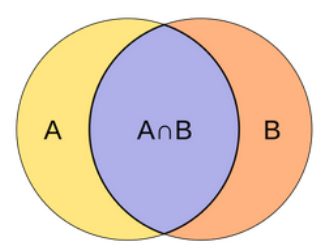
\includegraphics[width=0.6\textwidth]{3_iou.png}
	\caption[Caption for LOF]{Cách tính tỉ lệ IoU}
\end{figure}

\begin{center}
	\color{blue}
	A $\cap$ B / A $\cup$ B = A $\cap$ B / (area(A) + area(B) - A $\cap$ B)

\end{center}


\subsubsubsection*{Mục tiêu huấn luyện.} Mục tiêu của huấn luyện là giảm sai số điểm phân loại và sai số vị trí giữa box mẫu và box huấn luyện được lựa chọn từ chiến lược lựa chọn box mẫu. Do đó, hàm mất mát sẽ là tổng giữa hai sai số vị trí và sai số phân loại, theo công thức sau:
\begin{align} 
%\begin {center}
	L(x, c, l, g) = \dfrac{1}{N} \left (L_{conf} (x,c) + \alpha L_{loc} (x, l, g) \right)
 %\end{center}
\end{align} 

Trong đó

\begin{itemize}
	\item $x$ hay cụ thể là $x_{ij}^p = \{1; 0 \}$ là chỉ số cho biết box mặc định thứ i được gán cho
	box mẫu j có phân lớp p.
	\item $c$ là điểm phân loại
	\item $l$ là toạ độ box dự đoán
	\item $g$ là toạ độ box mẫu
	\item $\alpha$ là chỉ số cân bằng thể hiện quan hệ giữa $L_{conf}$ và $L_{loc}$
	\item $N$ là số lượng box mặc định đã được gán. Nếu $N$ $=$ $0$, thì sai số được gán bằng
	0
\end{itemize}

Hàm $L_{loc}$ sẽ được tính bằng hàm sai số Smooth L1 theo công thức cụ thể sau:

\begin{align} 
	%\begin {center}
		L_{loc}(x, l, g) = \sum_{i \in Pos}^N  \sum_{m \in (cx,cy,w,h))} x_{ij}^ksmooth_{L1}(l_i^m-\hat{g_j^m}) \\
		\hat{g_j^{cx}} = \dfrac{g_j^{cx}-d_i^{cx}}{d_i^w} \hspace{2cm} \hat{g_j^{cy}} = \dfrac{g_j^{cy}-d_i^{cy}}{d_i^h} \hspace{1.6cm}\\
		\hat{g_j^{w}} = log \left (\dfrac{g_j^{w}}{d_i^w} \right ) \hspace{2cm} \hat{g_j^{h}} = log \left (\dfrac{g_j^{h}}{d_i^h} \right ) \hspace{1.6cm}
	 %\end{center}
\end{align} 

Trong đó cx, cy, w, h lần lượt là toạ độ tâm, chiều rộng, chiều cao của box mặc định. \\
Hàm L conf sẽ được tính bằng công thức:
\begin{align} 
	%\begin {center}
		L_{con}(x, c) = - \sum_{i \in Pos}^N x_{ij}^plog(\hat{c_j^p}) - \sum_{i \in Neg} log(\hat{c_i^0}) \\
		\hat{c_i^p} = \dfrac{exp(c_i^p)}{\sum_p exp (c_i^p)} \hspace{2cm}
	 %\end{center}
\end{align}

\subsubsubsection*{Chọn độ lớn và tỉ lệ của hộp mặc định. }
Để giải quyết vấn đề kích thước đa dạng của các đối tượng có trong ảnh, SSD sử dụng bản đồ đặc trưng ở các lớp khác nhau để thực hiện dự đoán, cách này tương đương với việc huấn luyện ảnh ở nhiều kích thước khác nhau nhưng giảm khối lượng tính toán đi rất nhiều. SSD lựa chọn kích thước của các hộp mặc định theo phương thức như sau, giả sử sử dụng m bản đồ đặc trưng cho dự đoán, thì độ lớn của hộp mặc định tại mỗi bản đồ đặc trưng được cho bởi:\\
\begin{align}
	s_k = s_{min} + \dfrac{s_{max} - s_{min}}{m-1} (k-1), k \in [1, m]
\end{align}

Trong đó, 
\begin{itemize}
	\item $s_{min}$ = 0.2 và $s_{max}$ = 0.9, nghĩa là lớp thấp nhất sẽ có độ lớn 0.2 và lớp cao nhất sẽ
	có độ lớn 0.9 so với đối tượng gốc
\end{itemize}

Đồng thời, bằng nghiên cứu của mình, nhóm tác giả đã đặt ra các tỉ lệ mặc định khác
nhau $a_r \in \{1; 2; 3; 1 ; 1 \}$. \\

Từ đây, họ có thể  tính chiều rộng và chiều dài của box mặc định lần lượt là 
$s_k\sqrt{a_r}$ và $s_k / \sqrt{a_r}$. Trong trường hợp tỉ lệ là 1, họ thêm vào một box mặt định có
độ lớn $s_k' = \sqrt{s_k s_k + 1}$,  tổng cộng sẽ có 6 box mặt định cho mỗi vị trí (hay ô) trên bản đồ
đặc trưng. Tâm của mỗi box mặc định được tính bằng công thức 
$ \left ( \dfrac{i+0.5}{|f_k|}, \dfrac{j+0.5}{|f_k|} \right )$ , với $|f_k|$ là
kích thước của bản đồ đặc trưng thứ $k$ và $i$, $j$ $\in$ $[0; |f_k| ]$.

\subsubsubsection*{Khai thác mẫu âm.}
sau quá trình lựa chọn các hộp mặc định phục vụ quá trình huấn luyện, các hộp mặc định được chọn được gọi là mẫu dương, hầu hết các hộp mặc định sẽ không được chọn và những hộp mặc định này được coi là mẫu âm, đặc biệt khi số lượng hộp mặc định càng lớn thì số lượng mẫu âm này càng lớn. Điều này gây ra sự mất cân bằng giữa số lượng mẫu âm và số lượng mẫu dương (dễ bị miss - tỉ lệ bỏ sót cao). Thay vì sử dụng tất cả mẫu âm vào quá trình huấn luyện, SSD sắp xếp số mẫu âm này theo giá trị của hàm mất mát phân loại và lựa chọn ra những mẫu âm có mất mát lớn nhất để tham gia vào quá trình huấn luyện sao cho tỉ lệ giữa số lượng mẫu âm và số lượng mẫu dương là 3:1. Theo thực nghiệm, kỹ thuật này giúp quá trình tối ưu hàm mất mát nhanh hơn và ổn định hơn. 

\subsubsubsection*{Non-Maximum Suppression.}
Với thiết kế như trên, thì mô hình SSD vẫn còn một vấn đề, nhiều box dự đoán cùng chứa một đối tượng. 

\begin{wrapfigure}{r}[0pt]{0.3\linewidth}
	\includegraphics[scale=0.6]{3_nms.jpg}
	\caption[Caption for LOF]{Ví dụ về Non-Max Suppression \footnotemark[0]} 
\end{wrapfigure}
\footnotetext{Hình ảnh từ https://leonardoaraujosantos.gitbooks.io}

Như hình bên trái, nhiều bounding box cùng chứa khuôn mặt của đối tượng. Điều này làm cho kết quả của mô hình trở nên khó quan sát, không đảm bảo được độ chính xác của kết quả. Để giải quyết vấn đề này, mô hình ssd sử dụng thêm 1 bước hậu xử lý. Các output phải đi qua thêm 1 lớp non-maximum suppression. Ý tưởng chính của tầng này là lấy những box có confidence score cao nhất. Nếu có 1 box trong số này có IoU cao hơn 0.45 với bất kì box nào có cùng class từ những box đã lọc ở trên, box này sẽ bị loại bỏ.  \\

\subsubsubsection*{Làm giàu dữ liệu. } Vì ảnh trong tự nhiên là vô cùng đa dạng, phụ thuộc nhiều yếu tố bên ngoài như thời tiết, ánh sáng, bụi bẩn, .. rất khó để có thể chuẩn bị đủ dữ liệu huấn luyện cho tất cả các trường hợp. Sử dụng các kỹ thuật làm giàu dữ liệu làm cho tập dữ liệu huấn luyện lớn hơn, đa dạng hơn giúp cho mô hình "thông minh" hơn. Các kỹ thuật cơ bản: làm nhiễu, làm mờ, thay đổi kích thước ảnh, lật ảnh, .. 

\subsection{Mạng SSD512}
Mạng SSD 512 có cấu trúc giống SSD300 có 3 phần, base layers, extra layers và multibox layers
Tuy nhiên có một số điều chỉnh ở lớp extra layers và lớp multibox layers. Cụ thể,
\begin{itemize} 
\item Extra layers: Cấu trúc tương tự SSD 300 nhưng do kích thước đầu vào lớn, nên SSD512 
sẽ bổ sung thêm 2 layer ở cuối mạng.
\item Cũng tương tự SSD300 nhưng thay vì chỉ sử dụng 6 layer để tạo ra bounding box, SSD512 sử dụng 7 layers để tạo ra boungding box.
\end{itemize}

Từ những thay đổi so với SSD300, SSD512 mang lại những sự khác biệt cơ bản:
\begin{itemize} 
	\item Input lớn giúp SSD 512 tăng khả năng phát hiện các vật thể nhỏ hơn, phân tích ảnh đầu vào chi tiết hơn
	\item Có nhiều bounding box được sinh ra hơn nên tăng cao khả năng nhận diện được nhiều vật thể trong một frame ảnh.
	\item Tuy nhiên mạng này lại rất cồng kềnh so với SSD300, nên tốc độ inference kết quả rất chậm đề có thể chạy realtime.
\end{itemize}	

Chi tiết cấu trúc mạng SS512 sẽ được đề cập trong phần phụ lục. 

\section{Feature Fusion Single Shot MultiBox Detector}
SDD là một trong các giải thuật phát hiện và nhận dạng đối tượng tốt nhất hiện nay, bên cạnh YOLOv2 cả về độ chính xác và tốc độ. Tuy nhiên hạn chế lớn nhất của SSD là việc phát hiện các đối tượng có kích thước nhỏ do cấu trúc mạng có hình chóp và ảnh đầu vào cố định của nó chỉ có kích thước 300*300. Mạng SSD512 do hạn chế về tốc độ, chỉ bằng ~1/3 tốc độ SSD300.
\\

Có nhiều các tiếp cận khác nhau được đưa ra giải quyết vấn đề kích thước của đối tượng trong bài toán phát hiện và nhận dạng đối tượng như: chia nhỏ ảnh đầu vào, tích chập ngược mạng SSD (DSSD), cấu trúc lại mạng VGG, khai thác thông tin ngữ cảnh, ..
\\

Mô hình FSSD sử dụng kết hợp hai bản đồ đặc trưng để khai thác thông tin ngữ cảnh từ hình ảnh. thông tin về ngữ cảnh đặc biệt quan trọng với việc phát hiện đối tượng có kích thước nhỏ [1], vì đối tượng có kích thước nhỏ không có quá nhiều thông tin chi tiết (thông tin ngữ nghĩa - semantic information). Ví dụ đối với hình con thuyền trong hình 2.a, ngữ cảnh biển là đặc biệt quan trọng để giúp phát hiện đâu là con thuyền.
\\

\begin{figure}[h!]
	\centering
	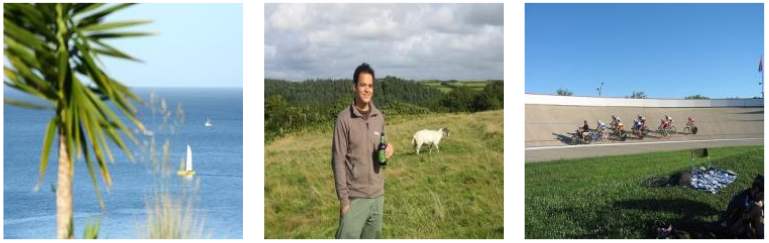
\includegraphics[width=0.6\textwidth]{3_contextual.png}
	\caption[Caption for LOF]{Sự tương quan giữa phát hiện đối tượng và ngữ cảnh trong ảnh}
	Việc phát hiện con thuyền trong ảnh 1.a sẽ khả thi hơn nếu nó xuất hiện trong ngữ cảnh là biển, tương tự việc phát hiện người cùng với xe đạp, hoặc chai nước trên tay người đàn ông. 
\end{figure}


Trong mạng SSD, nó sử dụng các lớp mạng nông để phát hiện các đối tượng nhỏ - Conv4\_3 và các lớp mạng nằm sâu hơn để phát hiện các đối tượng có kích thước lớn hơn. Tuy nhiên, các lớp mạng nông bị thiếu các thông tin ngữ cảnh nên dẫn đến sai lệch trong dự đoán. Làm thế nào để kết hợp thông tin ngữ cảnh được trích xuất ở các lớp mạng sâu hơn vào các lớp mạng nông hơn phát hiện đối tượng có kích thước nhỏ. 
\\

Một nhóm tác giả đề xuất xây dựng một module fusion, kết hợp thông tin giữa lớp mạng nông và lớp mạng nằm sâu hơn trong cấu trúc mạng SSD [2]. 
\cite{fssd}
\\

\begin{figure}[h!]
	\centering
	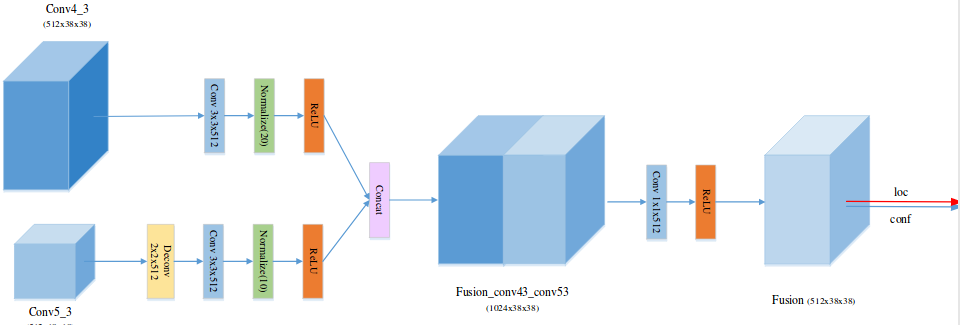
\includegraphics[width=0.6\textwidth]{3_fusion_module.png}
	\caption[Caption for LOF]{Khối concatenation}
\end{figure}

Như việc phân tích ở trên, các lớp mạng nằm sâu mang nhiều thông tin chi tiết hơn, nhiều thông tin ngữ cảnh hơn, làm thế nào để bổ sung thông tin này vào các lớp tích chập phát hiện đối tượng có kích thước nhỏ ở phía trước. 
\\

Để lựa chọn tầng mạng thích hợp để kết hợp, xem hình dưới. Feature map của lớp 4\_3 và 5\_3 là khá chính xác với đối tượng nhất. Conv3\_3 hầu như không có thông tin ngữ cảnh, còn Conv6 có quá nhiều thông tin có thể gây nhiễu. 
\\

\begin{figure}[h!]
	\centering
	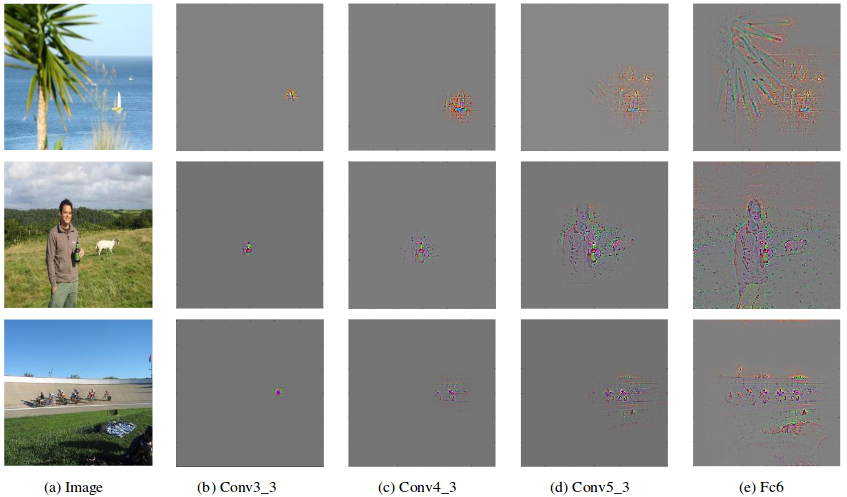
\includegraphics[width=1\textwidth]{3_conv_ef.png}
	\caption[Caption for LOF]{Phân tích Effective receptive fields trong kiến trúc SSD}
\end{figure}

Ưu điểm dễ thấy của FSSD là không làm thay đổi tốc độ của mạng FSSD, tuy nhiên thực nghiệm cho thấy, hiệu quả mà FSSD đem lại không thực sự cao.

\section{Single Shot Scale-invariant Face Detector }
Ưu điểm dễ thấy của FSSD là không làm thay đổi tốc độ của mạng FSSD, tuy nhiên thực nghiệm cho thấy, hiệu quả mà FSSD đem lại không thực sự cao.
\\
\subsection {Hạn chế của các mô hình phát hiện đối tượng. }
Các framework phát hiện đối tượng dựa vào các anchorbox thường bị bỏ sót các đối tượng có kích vừa hoặc nhỏ. Có hai nguyên nhân, thứ nhất, ở các lớp cuối cùng, qua rất nhiều lớp tích chập, thông tin của đối tượng còn rất ít hoặc bị mất đi, khiến mô hình không thể phát hiện đâu là đối tượng (1a). Nguyên nhân thứ hai là các đối tượng nhỏ, kích thước anchor box và receptive field không khớp (1b).
\\
%hình 
\begin{figure}[h!]
	\centering
	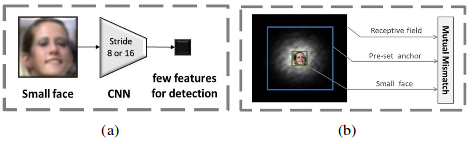
\includegraphics[width=0.6\textwidth]{3_erf.png}
	\caption[Caption for LOF]{Khối concatenation}
\end{figure}

Để giải quyết hai vấn đề trên, S3FD đề xuất một framework sử dụng các anchors có kích thước bằng nhau (scale-equitable), các anchor box được sắp xếp trên nhiều lớp với stride size từ 4 đến 128 pixel. Bên cạnh đó, S3FD sử dụng anchor box có scale từ 16 đến 512 pixel qua các lớp tương ứng với receptive field. Và khoảng cách giữa hai anchors kề nhau là cố định, đảm bảo anchors ở các lớp khác nhau khớp receptive field tương ứng và các anchors phân bố đều trên bức ảnh. 
\\

\subsection {Single shot scale-invariant face detector}
Ba đóng góp chính của S3FD có thể tóm tắt như sau:
\begin{enumerate}
\item Đề xuất một cấu trúc mạng mới cho bài toán phát hiện khuôn mặt dựa trên SSD và phương pháp lựa chọn kích thước anchor box hợp lý để giải quyết vấn đề kích thước đa dạng của đối tượng trong ảnh.
\item Chỉ ra chiến lược chọn các anchor box dương cho các đối tượng nhỏ trong ảnh để giảm tỉ lệ bỏ sót. (low recall rate) 
\item Giới thiệu kỹ thuật max-out background giúp giảm tỉ lệ phát hiện nhầm đối tượng nhỏ. 
Để phát hiện đối tượng có kích thước nhỏ thì phải đặt dày đặc các anchors có kich thước nhỏ, điều này dẫn đến tỉ lệ false positive tăng cao. Do đó để giảm tỉ lệ phát hiện nhầm này, S3FD đề xuất max-out background label cho lớp phát hiện ở nông nhất (trong S3FD là lớp Conv3\_3) 
\end{enumerate}

\begin{figure}[h!]
	\centering
	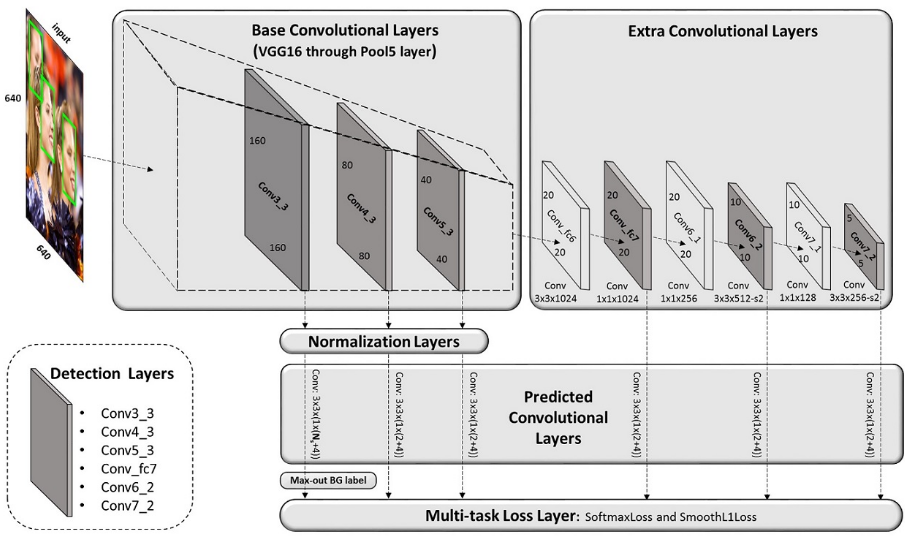
\includegraphics[width=1\textwidth]{3_s3fd_arch.png}
	\caption[Caption for LOF]{Kiến trúc mạng S$^3$FD \cite{s3sd}}
\end{figure}

\subsubsection{Scale-equitable framework}
\subsubsubsection*{Cấu trúc mạng.}
Dựa trên cấu trúc mạng SSD, S3FD sử dụng VGG16 làm lớp nền và bổ sung một số lớp tích chập khác. 

\begin{itemize}
\item Lớp nền:  giữ nguyên các lớp từ conv1\_1 đến pool\_5 của VGG16, và loại bỏ hết các lớp còn lại.
\item Lớp bổ sung: chuyển đổi hai lớp fc6 và fc7 của VGG16 thành các lớp tích chập bằng cách subsampling tham số của chúng [ref where] và thêm một số lớp tích chập như hình. Các lớp tích chập này kích thước giảm dần, các feature map cũng có kích thước giảm dần.
\item Lớp phát hiện: các lớp conv3\_3, conv4\_3, conv5\_3, conv\_fc7, conv6\_2 và conv7\_2 được chọn làm các lớp phát hiện, các lớp này sử dụng các anchor box có scale khác nhau để thực hiện việc phát hiện.
\item Lớp chuẩn hóa: Các lớp conv3\_3, conv4\_3 và conv5\_3 có feature scale khác nhau. Do đó sử dụng chuẩn hóa L2 để rescale their norm to 10, 8 và 5, các tham số scale này được học trong suốt quá trình lan truyền ngược.
\item Lớp dự đoán: Mỗi lớp phát hiện được gắn vào một lớp tích chập có kích thước px3x3xq với p là số lượng kênh của đầu vào và đầu ra, 3x3 là kích thước kernel. Với mỗi anchor, S3FD dự đoán 4 tham số liên quan tới tọa độ và Ns các điểm cho bài toán phân loại, trong đó Ns = Nm + 1 (Ns là max-out backgroundth label) đối với lớp conv3\_3 và Ns = 2 cho các lớp các lại. Chú ý đang xét bài toán gốc của bài báo là phát hiện khuôn mặt nên chỉ có hai lớp cần phân loại là face và nonface.
\item Lớp mất mát: S3FD sử dụng sofmax loss cho bài toán phân loại và smooth L1 loss cho bài toán hồi quy.
\end{itemize}

\subsubsubsection*{Kích thước của các anchor box.}

Sáu lớp phát hiện sử dụng các anchor box có scale khác nhau, tương ứng trong bảng 1. Trong s3fd, các anchor box đều sử dụng aspect ratio 1:1 để phát hiện khuôn mặt, nhóm sẽ tùy chỉnh là tỉ lệ aspect ratio này để áp dụng vào bài toán phát hiện nhiều đối tượng của nhóm. 
\begin{itemize}
\item effective receptive field: trong một mạng tích chập có hai loại receptive field, một là theoretical receptive field chỉ toàn bộ vùng điểm ảnh trong ảnh đầu vào ảnh hưởng đến kết quả đầu ra của mạng CNN. Nhưng trên thực tế, chỉ có những điểm ảnh nằm ở vùng trung tâm mới gây ảnh hưởng rõ ràng đến giá trị đầu ra. Vùng điểm ảnh trung tâm này khá nhỏ so với theoretical receptive field và nó được gọi là effective receptive field. Như vậy, anchor box nên được chọn nhỏ hơn theoretical receptive field để có thể khớp với effective receptive field nhất. 
\item equal-proportion interval principle: stride size sẽ được lựa chọn dựa trên anchor scale, và tỉ lệ stridesize/anchor luôn bằng 1/4. ĐIều này đảm bảo các anchor có scale khác nhau phân bố đều trên ảnh, cơ hội các box này khớp với đối tượng có kích thước đa dạng lớn hơn.
\end{itemize}

\begin{table}[h!]
	\centering
	\caption{chưa biết ghi gì}
	\begin{tabular}{|cccc|}
		\hline
		Detection Layers & Stride & Anchor & RF \\ \hline
		conv3\_3 & 4 &16& 48 \\ 
		conv4\_3  & 8 &32& 108 \\
		conv5\_3 &16 &64 &228 \\
		conv\_fc7 &32 &128 &340 \\
		conv6\_2 &64 &256& 468 \\
		conv7\_2 &128& 512& 724 \\ \hline
	\end{tabular}
\end{table}

\subsubsection{Scale compensation anchor matching strategy}
Trong phương pháp huấn luyện của SSD, người ta tìm các anchor box có jaccard overlaped với groundtruth lớn hơn một ngưỡng nào đó. Tuy nhiên, kích thước anchor box thuộc miền rời rạc trong khi đó kích thước khuôn mặt trong ảnh tự nhiên thuộc miền liên tục, do đó có rất nhiều khuôn mặt không khớp với anchor box, chính điều này dẫn đến tỉ lệ recall thấp (tỉ lệ bỏ sót cao). Để giải quyết vấn đề này, s3fd đề xuất giải pháp có hai giai đoạn:
quan hệ giữa kích thước đối tượng và số lượng anchor box khớp với đối tượng.
\\
\begin{wrapfigure}{r}[0pt]{0.4\linewidth}
	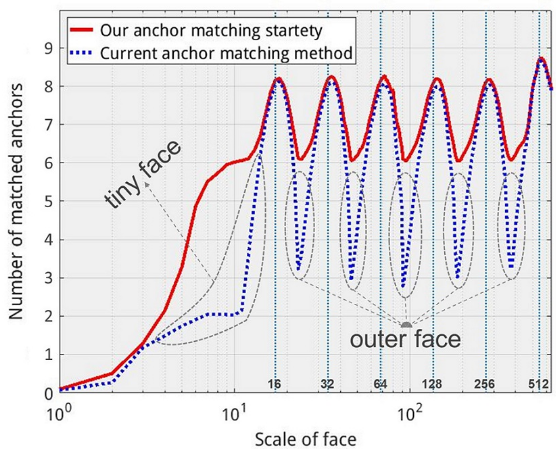
\includegraphics[scale=0.35]{3_facescale.png}
	\caption[Caption for LOF]{Facescale \footnotemark[0]} 
\end{wrapfigure}
\textbf{Giai đoạn một}: Ở bài toán phát hiện thông thường, ngưỡng jaccard overlap thường là 0.5. Nhưng đối với các đối tượng có kích thước nhỏ, tỉ lệ giao với anchorbox rất khó đạt được 0.5. Do đó, s3fd đề nghị giảm ngưỡng này xuống 0.35 nhằm tăng số lượng anchor box khớp với đối tượng.
\\

\textbf{Giai đoạn hai}: Sau khi thực hiện giai đoạn một, một vài đối tượng vẫn không khớp với bất kì anchor box nào hoặc khớp không đủ số anchor box dương trung bình. S3FD thực hiện giai đoạn hai: lựa chọn ra những anchor box có jaccard overlap với đối tượng đó lớn hơn 0.1, tiếp tục sắp xếp lại và chọn ra những box có jaccardoverlap cao nhất.

\subsubsection{Max-out background label.}
Trong mô hình s3fd, số lượng anchor box khởi tạo là rất lớn, có hơn 34125 box trong khi đối tượng trên ảnh chiếm một phần rất nhỏ, điều này dẫn đến sự mất cân bằng khi thực hiện phân loại. Số lượng box nhỏ chủ yếu tập trung ở lớp conv3\_3, có hơn 75 tổng số anchor box tập trung ở lớp này, sự mất cân bằng này dẫn tới tỉ lệ false positve cao, đặc biệt tỉ lệ báo động nhầm ở các box nhỏ nhất. 
\\

\begin{wrapfigure}{r}[0pt]{0.4\linewidth}
	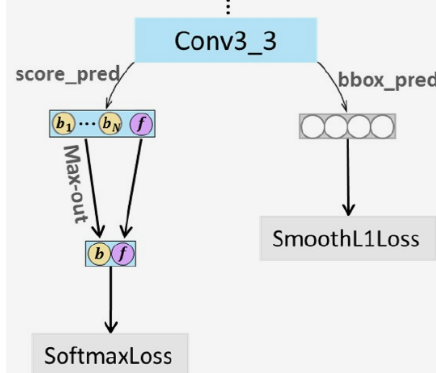
\includegraphics[scale=0.35]{3_maxout.png}
	\caption[Caption for LOF]{Facescale \footnotemark[0]} 
\end{wrapfigure}

Để giải quyết vấn đề này, tác giả s3fd đề xuất một kỹ thuật gọi là max-out background vào lớp conv3\_3. Với mỗi anchor box, thay vì dự đoán 1 nhãn background và các nhãn còn lại, s3fd có Nm>1 điểm cho nhãn background và chọn ra điểm score cao nhất cho trong số Nm điểm này để đưa vào hàm tính mất mát. 



\chapter{NỘI DUNG THỰC HIỆN}
\section{Mục tiêu} thử nghiệm các mô hình và giải pháp cải tiến, sau đó triển khai lên computing box
\section{Thử nghiệm các mô hình}
\subsection{Chuẩn bị dữ liệu}
\subsection{Một số tham số cần lưu ý}
\subsection{Đánh giá mô hình}
\subsection{Tối ưu hàm mất mát}

\section{Triển khai mô hình lên board Jetson}
\subsection{Hướng triển khai}
Trong phạm vi luận văn và điều kiện vật chất không cho phép, nhóm chỉ tiến hành triển khai mô hình SSD300 lên Jetson TX2. Nhóm sẽ triển khai SSD theo hai cách: thứ nhất sẽ triển khai mô hình với caffe; thứ hai nhóm sẽ triển khai và tối ưu hóa mạng bằng TensorRT và tiến hành đánh giá hiệu năng.
\subsection{Giới thiệu về Jetson TX2}
Jetson TX2 là một máy tính nhúng được NVDIA phát triển. Nó có khả năng triển khai và chạy các ứng dụng AI ngay trên chính nó (delivering AI at Edge) với mức tiêu hao năng lượng thấp. 
\\

\begin{figure}[h!]
	\centering
	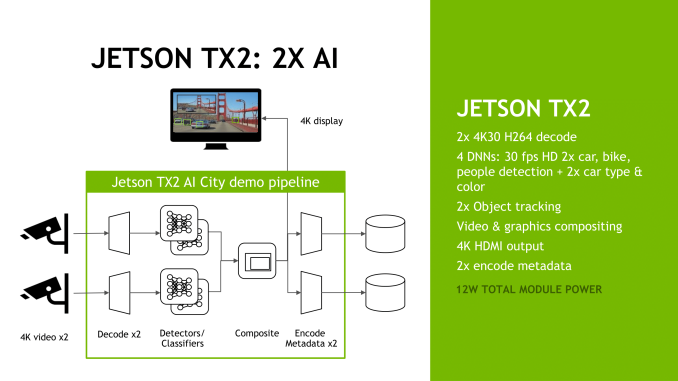
\includegraphics[width=1\textwidth]{4_2_tx2.png}
	\caption{Jetson TX2 trong phát triển thành phố thông minh}
\end{figure}

Jetson TX2 có sức mạnh gấp đôi so với người tiền nhiệm là Jetson TX1. Jetson TX2 mang trong mình là NVIDIA Pascal GPU với 256 cores. Cùng với đó là 2 CPU Cluster ARM v8 64bits được kết nối với nhau. Trong đó, Dever 2 (Dual-Core) được tối ưu hóa cho ứng dụng đơn luồng, còn ARM Cortex-A57 Quadcore thích hợp cho các ứng dụng đa luồng. Jetson TX 2 hỗ trợ mã hóa và giải mã video bằng phần cứng với chất lượng video tối đa là 4K/60Fps. Ngoài ra, Jetson TX2 cũng hỗ trợ các kết nối cơ bản như Wifi, Bluetooth, ethernet, …. \\

\begin{figure}[h!]
	\centering
	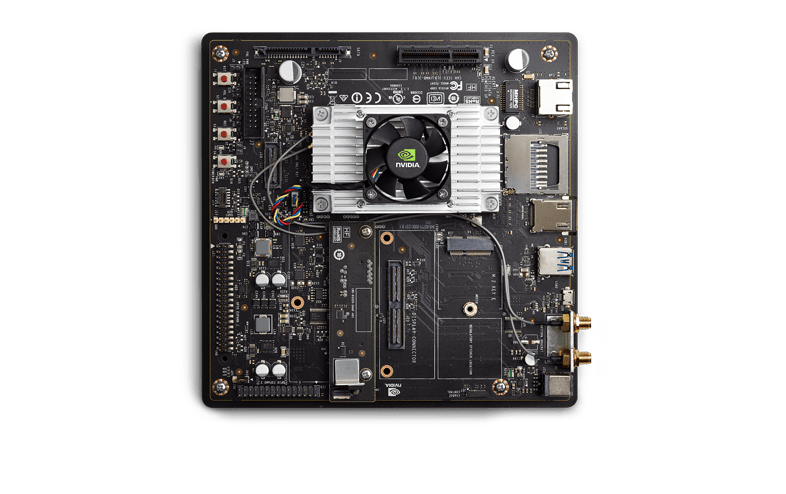
\includegraphics[width=1\textwidth]{4_2_kit.png}
	\caption[Kit phát triển Jetson TX2]{Đi cùng với Jetson TX2 là board mở rộng, hỗ trợ các cổng giao tiếp cơ bản giúp nhà phát triển giao tiếp với TX2.}
\end{figure}

Là một máy tính nhúng, năng lượng tiêu thụ là vấn đề quan trọng cần được chú ý. TX2 có thể điều chỉnh cấu hình dựa vào năng lượng tiêu thụ. TX2 hỗ trợ 2 chế độ hoạt động và MAX-Q và MAX-P. MAX-Q là chế độ hoạt động tiết kiệm năng lượng với công suất tiêu thụ là 7.5W trong khi đó MAX-P là chế độ hoạt động mang lại hiệu năng cao nhất với công suất chỉ 15W.\\

Bên cạnh đó, với kích thước nhỏ gọn (50mm*87mm) Jetson TX2 mang đầy đủ các yếu tố để phát triển các ứng dụng AI -  DeepLearning đòi hỏi khả năng tính toán cao với mức tiêu thụ năng lượng thấp, thích hợp với để phát triển computing box thực hiện tính toán thời gian thực tại cạnh (at the edge) trong mô hình “edge computing”.
\\

Đi cùng với các dòng Jetson là NVIDIA Jetpack SDK – bộ công cụ cung cấp các giải pháp cho việc phát triển và xây dựng các ựng dụng AI trên Jetson. Trong phạm vi luận văn lần này, nhóm sử dụng Jetpack phiên bản 3.2. Bộ Jetpack 3.2 bao gồm:
\begin{itemize}
\item OS Image: L4T 28.2 trên nền Ubuntu 16.04
\item Các bộ thư viện:
\begin{itemize}
	\item CUDA 9.0 Toolkit
	\item 	cuDNN v7.0.5
	\item 	OpenCV 3.3.1
	\item 	TensorRT 3.0
	\item 	VisionWorks
\end{itemize}
\item Các công cụ để phát triển:
\begin{itemize}
	\item  NVIDIA System Profiler
	\item  Tegra Graphics Debugger
\end{itemize}
\end{itemize}

\subsection{TensorRT}
NVIDIA TensorRT là công cụ tối ưu hóa quá trình “inference” cho các ứng dụng deep learning. Quá trình “Inference” là khi truyền mẫu dữ liệu mới vào mô hình mạng đã được học và đưa ra kết quả dự đoán hay phân loại. Quá trình này trong “machine learning” còn được gọi là “prediction” hay “scoring”. Mô hình đã được huấn luyện thường chạy như một “web-service” đáp ứng hàng triệu yêu cầu (request) từ người dùng đồng thời, sau đó thực hiện quá trình “inference” và trả kết qủa về cho người dùng. Để mang lại trải nghiệm cho người dùng, tất cả các quá trình trên cần phải có độ trễ (latency) thấp. Tương tự, đối với các thiết bị như xe tự hành thì khả năng đáp ứng thời gian thực (real-time) là một yêu cầu tối quan trọng cần phải đạt được để đảm bảo đố an toàn cho người sử dụng. Bên cạnh đó thì yêu cầu về năng lượng cũng cần phải được tính đến để tăng thời gian sử dụng giữa các lần “sạc”.
Về cơ bản, các ứng dụng AI nói chung, “deep learning” nói riêng cần phải đáp ứng được các yêu cầu sau:
\begin{itemize}
	\item Thông lượng cao (High throughput): các ứng dụng cần phải xử lí đồng thời một lượng lớn dữ liệu từ nhiều người dùng cùng một lúc.
	\item Độ trễ thấp (Low response time)
	\item Hiệu quả năng lượng
	\item Giải pháp triển khai đơn giản, gọn nhẹ, ít bị phụ thuộc vào môi trường phát triển.
\end{itemize}

NVIDIA TensorRT giải quyết các yêu cầu trên bằng cách tối ưu hóa các mô hình đã được huấn luyện để đưa ra một “inference engine” có thể đạt được hiệu năng cao trên GPU. Quá trình triển khai một mô hình với TensorRT bao gồm 2 bước chính:
\begin{itemize}
	\item Tối ưu mô hình được đưa vào và sinh ra “inference engines”: Sử dụng TensorRT để phân tích mô hình được đưa vào, tối ưu mô hình cho nền tảng được triển khai. Kết quả là bước này là “inference engine” được tối ưu từ các mô hình và được lưu lại trên đĩa.
	\begin{figure}[h!]
		\centering
		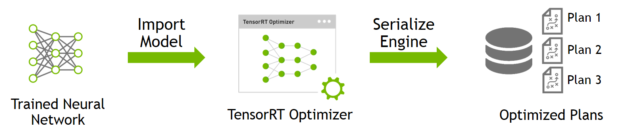
\includegraphics[width=1\textwidth]{4_2_infermodel.png}
		\caption{Tối ưu hóa mô hình}
	\end{figure}

	\item Triển khai “inference engine”.
	\begin{figure}[h!]
		\centering
		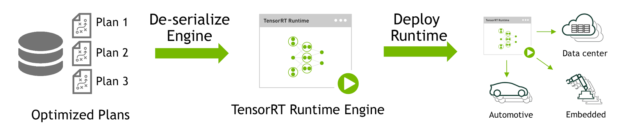
\includegraphics[width=1\textwidth]{4_2_infermodel2.png}
		\caption{Triển khai mô hình đã được tối ưu}
	\end{figure}
\end{itemize}
\subsubsection{Mô hình đầu vào}
Hiện nay, có rất nhiều “deep learning framework”, mỗi framework lại có một cấu trúc mạng “neural network” riêng biệt và định dạng khác nhau. Đối với Caffe và TensorFlow, TensorRT cung cấp sẵn C++ và Python API để đưa mô hình đã được huấn luyện vào để tối ưu hóa.\\

\begin{figure}[h!]
	\centering
	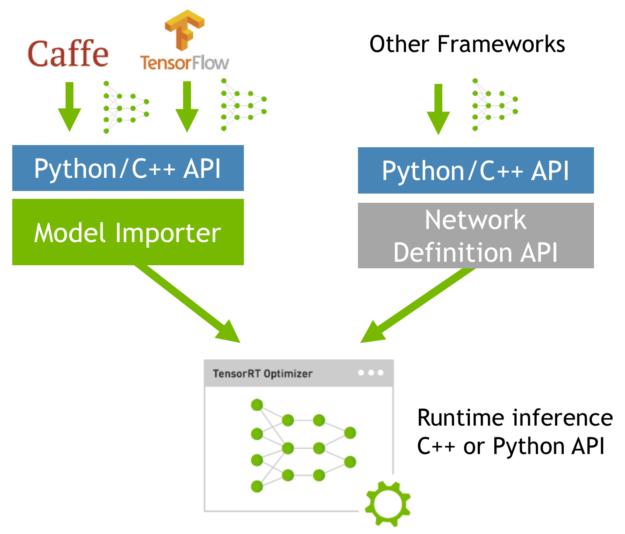
\includegraphics[width=0.8\textwidth]{4_2_import.png}
	\caption{Import mô hình vào TensorRT}
\end{figure}


Đối với các framework khác, người dùng có thể sử dụng “TensorRT’s Network Definition API” để mô tả và tải mô hình vào TensorRT.
\begin{itemize}
	\item TensorRT hỗ trợ các kiến trúc mạng thông dụng sau:
	\item Convolution
	\item LSTM và GRU
	\item Các hàm truyền: ReLU, tanh, sigmoid
	\item Pooling: max và average
	\item Scaling
	\item Element wise operation
	\item LRN
	\item Fully-connected
	\item SoftMax
	\item Decovolution
\end{itemize}

Tuy nhiên, “deep learning” đang phát triển hàng ngày và các kiến trúc mới thường xuyên được giới thiệu. Bởi vậy, TensorRT cung cấp “Custom Layer API (C++)” cho phép người dùng định nghĩa các lớp (layer) theo nhu cầu sử dụng mà TensorRT không hỗ trợ.

\subsubsection{Tối ưu hóa mô hình với TensorRT}
Khi mô hình được đưa vào, TensorRT sẽ tự động tối ưu hóa theo các tiêu chí sau:
\begin{itemize}
	\item Kết hợp các layer và loại bỏ các layer không được sử dụng
	\item Hiệu chỉnh tính chính xác(precision) từ FP32 (Float 32bit) về FP16 hoặc INT8 (integer 8bit)
	\item Điều chỉnh tham số (autotunnng)
	\item Sử dụng hiệu quả bộ nhớ
\end{itemize}

\begin{figure}[h!]
	\centering
	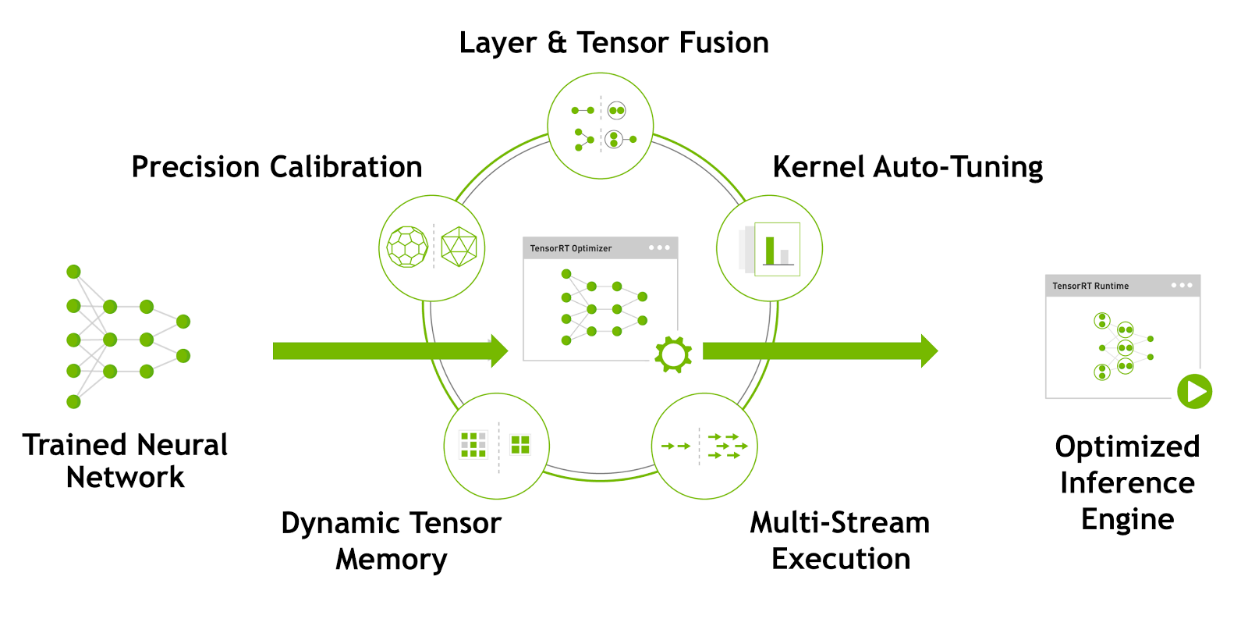
\includegraphics[width=0.8\textwidth]{4_2_optim.png}
	\caption{Quá trình tối ưu trên TensorRT}
\end{figure}

Việc tối ưu này cần được thực hiện ngay trên chính nền tảng sẽ triển khai. Ví dụ như để triển khai “inference” trên Jetson TX2 thì giai đoạn tối ưu cần phải được chạy trên Jetson TX2.
\begin{itemize}
	\item Kết hợp các lớp (layer)

\end{itemize}

TensorRT phân tích kiến trúc mô hình được dứa vào và tìm cách tối ưu nó. Việc tối ưu sẽ không làm thay đổi tính toán bên dưới mà thay vào đó chỉ tái cấu trúc lại mô hình để việc tính toán nhanh va hiệu quả hơn.
\begin{figure}[h!]
	\centering
	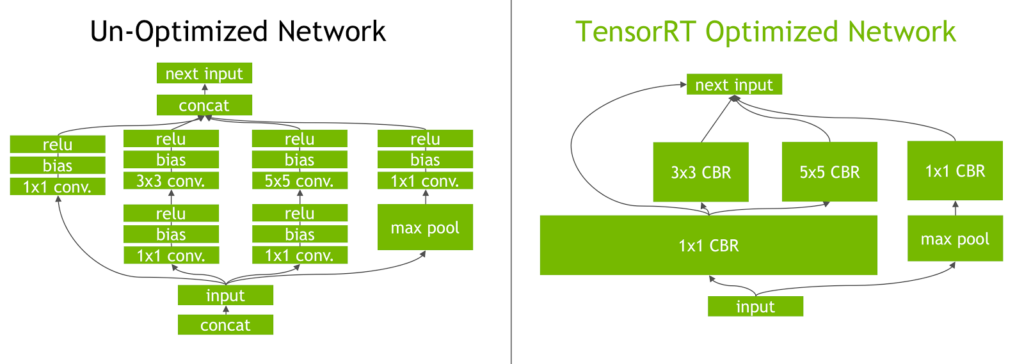
\includegraphics[width=0.8\textwidth]{4_2_combine.png}
	\caption{Kết hợp các lớp theo chiều dọc và chiều ngang}
\end{figure}

Trong quá trình “inference”, tính toán trên GPU (CUDA kernel) thường diễn ra rất nhanh nhưng quá trình đọc ghi dữ liệu lại rất tốn chi phí (overhead). Điều này dẫn đến tinh trạng nghẽn cổ chai (bottleneck) và sẽ không tận dụng hết hiệu năng tính toán của GPU. TensorRT giải quyết vấn đề này bằng cách kết hợp các kernel theo chiều dọc để thực hiện cùng nhau. Điều này hạn chế việc đọc ghi dữ liệu giữa các layer với nhau. Ví dụ, các lớp “convolution”, “relu”, “bias” có thể kết hợp với nhau thành một lớp duy nhất. Bên cạnh đó, các kernel có cùng dữ liệu đầu vào và kích thước bộ lọc (filter) cũng có thể kết hợp lại một lớp duy nhất (theo chiều ngang). \\

\begin{table}[h!]
	\centering
	\caption{Số lớp (layer) của một số mô hình trước và sau khi tối ưu.}
	\begin{tabular}{|ccc|}
		\hline
		Network & Layers & Layers after Fusion \\ \hline
		VGG19 & 43 & 27\\ 
		Inception V3  & 209 & 113 \\
		ResNet-152 & 670 & 159 \\ \hline
	\end{tabular}
\end{table}

\begin{itemize}
	\item Hiệu chỉnh chính xác về  FP16 và INT8.\\
	Hầu hết các “deep learning framework” trong quá trình huấn luyện mô hình sẽ sử dụng FP32. Tuy nhiên do yêu cầu về độ trể, quá trình tính toán có thể sử dụng FP16 hoặc cả INT8 (Jetson TX2 không hỗ trợ), bởi vì việc tính đạo hàm không được yêu cầu. Sử dụng FP16 hay INT8 mang lại thời gian tính toán nhanh hơn nhưng yêu cầu ít không gian lưu trữ hơn.
	\item Hiệu chỉnh tham số (auto tunning).\\
	TensorRT sẽ điều chỉnh các tham số để tối ưu trên nền tảng được triển khai bao gồm kích thước dữ liệu đâu vào, kích thước bộ lọc và các tham số khác
	\item Vùng nhớ động (Dynamic Tensor Memory).\\
	TensorRT cũng làm giảm lượng bộ nhớ và cải thiện khả năng tái sử dụng bộ nhớ bằng cách chỉ định bộ nhớ cho mỗi tensor chỉ trong suốt thời gian sử dụng, tránh chi phí cấp phát bộ nhớ để thực thi nhanh và hiệu quả
\end{itemize}

\subsection{Triển khai mô hình SSD300 với TensorRT}
TensorRT v3.04 hỗ trợ các bộ thư viện deep learning bao gồm Caffe, Pytoch, Tensorflow. Tuy nhiên Pytorch và TensorFlow chỉ được hỗ trợ đối với hệ máy x86. Vì vậy, nhóm sẽ triển khai SSD với TensorRT bằng mô hình đã được huấn luyện với Caffe. \\

Ngoài các lớp (layer) được TensorRT hỗ trợ, nhóm phải hiện thực các lớp sau với “Custom Layer API (C++)
\begin{itemize}
	\item Lớp Concat: TensorRT chỉ hỗ trợ trong trường hợp axis=1. Nên nhóm phải hiện thực lại trong trường hợp axis=2.
	\item Lớp Softmax: Tương tự với lớp Concat, nhóm cũng cần phải hiện thực lại lớp Softmax với axis=2.
	\item Lớp Reshape.
	\item Lớp Flatten.
\end{itemize}

Sau khi hiện thực xong các lớp, quá trình hoạt động của TensorRT trên TX2 bao gồm các bước:
\begin{itemize}
	\item Tải mô hình caffe đã được huấn luyện cùng với cấu trúc mạng vào TensorRT: tệp mô tả cấu trúc mạng (prototxt) sẽ được chỉnh sửa cho phù hợp để đưa vào TensorRT. 
	\item Chuyển đổi từ caffe sang “TensorRT engine”: tại đây có thể chọn FP32 hoặc FP16. TX2 không hỗ trợ đối với INT8.
	\item Đưa dữ liệu từ camera vào “TensorRT engine” để tiến hành “inference”: output bao gồm nhãn của box, confident và vị trí của box.
\end{itemize}

Cách sử dụng sẽ được hướng dẫn chi tiết tại Phụ lục.
\subsection{Triển khai mô hình SSD với Caffe}
Chi tiết cách triển khai mô hình SSD với Caffe trên TX2 tham khảo Phụ lục:
\subsection{Kêt quả thực nghiệm}
Trong quá trình thực nghiệm, nhóm sẽ sử dụng mô hình SSD300 được huấn luyện trên tập dữ liệu “VOC0712” và “COCO” của Wei Liu.
Nhóm sẽ tiến hành đánh giá tốc độ xử lí của Jetson TX2 đối với mô hình SSD300 sử dụng camera được tích hợp sẵn trên board trong các trường hợp sau:

\begin{itemize}
	\item Trường hợp 1: Mô hình SSD được triển khai bằng thư viện Caffe.
	\item Trường hợp 2: Mô hình SSD đã được tối ưu hóa bằng TensorRT dùng FP32.
	\item Trường hợp 3: Mô hình SSD đã được tối ưu hóa bằng TensorRT dùng FP16.
\end{itemize}
Kêt quả nhóm thu được trong các trường hợp như sau:
\begin{table}[h!]
	\centering
	\caption{Số lớp (layer) của một số mô hình trước và sau khi tối ưu.}
	\begin{tabular}{|c|c|}
		\hline
		  & Frames per second \\ \hline
		Trường hợp 1 & 4 fps \\ \hline
		Trường hợp 2 & 7 fps \\ \hline
		Trường hợp 3 & 11 fps \\ \hline
	\end{tabular}
\end{table}

	\begin{figure}[h!]
		\centering
		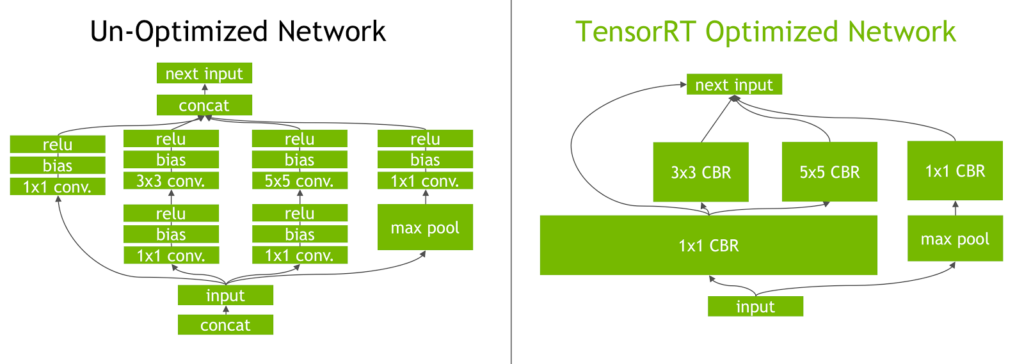
\includegraphics[width=0.8\textwidth]{4_2_combine.png}
		\caption{Hình ảnh từ quá trình thực nghiệm}
	\end{figure}
	Từ kết quả trên ta thấy đối với với mô hình SSD300 được tối ưu hóa bằng TensorRT với FP16 đạt tốc độ gấp gần 3 lần so với mô hình được triển khai chỉ bằng thư viện caffe trong khi độ chính xác là tương đương nhau, đáp ứng được yêu cầu chạy với thời gian thực\\



\chapter{KẾT LUẬN, ĐÁNH GIÁ, HƯỚNG PHÁT TRIỂN}


%%%chú thích 
<abc>
\footnote{là abcd}

%%%insert ảnh, nhớ captioning và ghi nguồn 
%-------------Figure 2 ---------------------------------
%\begin{figure}[h!]
%	\centering
%	\includegraphics[width=0.8\textwidth]{anm_victim_destop2.PNG}
%	\caption{Tình trạng máy nạn nhân sau cuộc tấn công}
%	\end{figure}
	
%%%%%%%%%%%%%%%%%

\begin{figure}[h!]
	\centering
	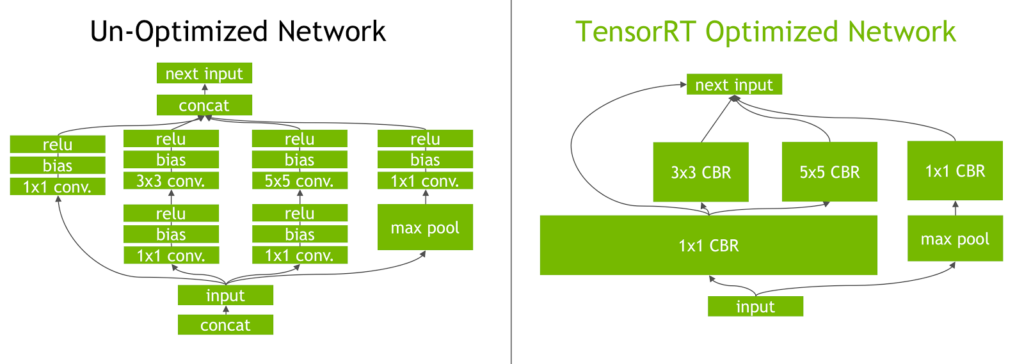
\includegraphics[width=0.8\textwidth]{4_2_combine.png}
	\caption{Hình ảnh từ quá trình thực nghiệm}
\end{figure}

%{PHỤ LỤC}
%%%%%%%%%%%%%%%%%%%
%% cài đặt jetson tx2
\textbf{Tải jetpack 3.2} tại trang chủ của Nvidia
\begin{center}
\color{blue}
https://developer.nvidia.com/jetson-development-pack
\end{center}

\textbf{Cài đặt jetpack 3.2} 
\begin{itemize}
	\item Đầu tiên, kết nối cáp Ethernet giữa Jetson-board với máy tính linux hoặc cùng một router với máy tính linux
	\item Thêm quyền thực thi cho  JetPack-{VERSION}.run đã tải bằng câu lệnh:
		\begin{lstlisting}[language=bash, frame=single]
			$ chmod +x JetPack-{VERSION}.run
		\end{lstlisting}
	\item Chạy JetPack-{VERSION}.run bằng câu lệnh:
		\begin{lstlisting}[language=bash, frame=single]
			$ ./ JetPack-${VERSION}.run
		\end{lstlisting}

	
		Jetpack LT4 Installer được khởi động như sau:
	\item Chọn thư mục cài đặt và ấn next.
	\item Chọn môi trường cài đặt, chọn Jetson TX2.
	\item Jetpack Installer sẽ yêu cầu quyền sudo cho quá trình cài đặt.
	\item Chọn các gói thư việc muốn cài đặt, mặc định là sẽ cài đặt tất cả.
	\item Chấp nhận các chính sách của Nvidia.
	\item Trình cài đặt sẽ tải và cài đặt các gói thư viện. Khi hoàn thành  chọn Next để đến bước tiếp theo.
	\item Nếu không chọn Flash OS trong bước Component Manager thì nhập IP, user name và password của jetson.
	\item Ngược lại, nếu chọn Flash OS trong bước Component Manager, chọn mô hình mạng kết nối ban đầu ( trong trường hợp này là kết nối với chung router) 
	\item Chọn cách thức host kết nối với router (wireless hay ethernet)
	\item Một cửa sổ hướng dẫn chuyển Jetson qua chế độ Force USB Recovery Mode. Thực hiện theo hướng dẫn để Flash OS.
	\item Sau khi chuyển qua chế độ Force USB Recovery Mode sẽ tiến hành Flash OS và cài đặt các gói thư viện.
	\item Cài đặt hoàn tất.
\end{itemize}

\textbf{Cài dặt OpenCV 3.0}
Jetpack 3.2 (hoặc 3.1) có sẵn OpenCv nhưng chỉ hỗ trợ cho python2, do đó cần phải cài đặt lại OpenCV cho python3.
Để cài đặt OpenCv cho python 3, sử dụng các câu lệnh sau:
\begin{lstlisting}[language=bash, frame=single]
	$ sudo apt-get install build-essential make cmake cmake-curses-gui\
                       g++ libavformat-dev libavutil-dev \
                       libswscale-dev libv4l-dev libeigen3-dev \
                       libglew1.6-dev libgtk2.0-dev

	$ sudo apt-get install libdc1394-22-dev libxine2-dev \
						libgstreamer1.0-dev \
						libgstreamer-plugins-base1.0-dev

	$ sudo apt-get install libjpeg8-dev libtiff5-dev libjasper-dev \
						libpng12-dev libavcodec-dev

	$ sudo apt-get install libxvidcore-dev libx264-dev libgtk-3-dev \
						libatlas-base-dev gfortran

	$ sudo apt-get install python3-dev python3-pip
	$ sudo pip3 install numpy

	$ sudo apt-get install python-dev python-pip
	$ sudo pip install numpy

	$ mkdir -p ~/src
	$ cd ~/src
	$ wget https://github.com/opencv/opencv/archive/3.3.1.zip

	$ cd opencv-3.3.0
	$ mkdir build
	$ cd build
	$ cmake -D CMAKE_BUILD_TYPE=RELEASE -D CMAKE_INSTALL_PREFIX=/usr/local \
			-D WITH_CUDA=ON -D CUDA_ARCH_BIN="6.2" -D CUDA_ARCH_PTX="" \
			-D WITH_CUBLAS=ON -D ENABLE_FAST_MATH=ON -D CUDA_FAST_MATH=ON \
			-D ENABLE_NEON=ON -D WITH_LIBV4L=ON -D BUILD_TESTS=OFF \
			-D BUILD_PERF_TESTS=OFF -D BUILD_EXAMPLES=OFF ..
	$ make -j4
	$ sudo make install
\end{lstlisting}

Sau khi cài đặt OpenCv, có thể dùng python3 để sử dụng camera mặc định của Developer Kit hiện thị trên màn hình. Tải ví dụ tại: 
\begin{center}
\color{blue}
https://gist.github.com/jkjung-avt/86b60a7723b97da19f7bfa3cb7d2690e 
\end{center}
Chạy code với câu lệnh:
\begin{lstlisting}[language=bash, frame=single]
	$ python3 tegra-cam.py
\end{lstlisting}

\textbf{cài đặt caffee và pycaffee}
Caffe là deep learning framework được hỗ trợ tốt nhất bởi TensonRT. Vì vậy sử dụng Caffe sẽ tối ưu hóa hiệu năng của Jetson Tx2.
Trước khi cài đặt Caffe, cần phải cài đặt thành công OpenCv. Tiếp theo cài đặt các thư viện phụ thuộc sau:
\begin{lstlisting}[language=bash, frame=single]
	$ sudo apt-get install libprotobuf-dev libleveldb-dev libsnappy-dev libhdf5-serial-dev protobuf-compiler
	$ sudo apt-get install --no-install-recommends libboost-all-dev
	$ sudo apt-get install libgflags-dev libgoogle-glog-dev liblmdb-dev
	$ sudo apt-get install libatlas-base-dev
	$ sudo apt-get install python3-dev
\end{lstlisting}

Sau đó, tải caffe từ github và cài đặt từ source đã tải về:
\begin{lstlisting}[language=bash, frame=single]
	$ cd ~
	$ git clone https://github.com/BVLC/caffe
	$ cd caffe
\end{lstlisting}

Tải Makefile.config và copy vào thư mục caffe:
\begin{center}
\color{blue}
https://jkjung-avt.github.io/assets/2017-08-08-caffe-on-tx2/Makefile.config
\end{center}

Tiến hành compile Caffe từ Makefile:

\begin{lstlisting}[language=bash, frame=single]
	$ make -j4 all
	$ make -j4 test
	### Test and verify the caffe build
	$ make runtest
\end{lstlisting}

Cài đặt caffe cho python3 bằng những câu lệnh sau:

\begin{lstlisting}[language=bash, frame=single]
	$ sudo apt-get install python3-pip
	$ sudo pip3 install --upgrade pip
	$ sudo pip3 install --upgrade setuptools
	$ sudo pip3 install -r ~/caffe/python/requirements.txt

	$ sudo pip3 install --upgrade python-dateutil
	$ sudo pip3 install protobuf
	$ cd ~
	$ mkdir -p src
	$ cd src
	### Build and install leveldb-0.20
	$ wget https://pypi.python.org/packages/03/98/1521e7274cfbcc678e9640e242a62cbcd18743f9c5761179da165c940eac/leveldb-0.20.tar.gz

	$ tar xzvf leveldb-0.20.tar.gz
	$ cd leveldb-0.20
	$ python3 setup.py build
	$ sudo python3 setup.py install
	### Build and install matplotlib (2.0.2)
	$ cd ~/src
	$ git clone https://github.com/matplotlib/matplotlib.git
	$ cd matplotlib
	$ python3 setup.py build
	$ sudo python3 setup.py install
	$ sudo apt-get install tcl-dev tk-dev
	$ sudo pip3 install pytk
	### Final step: modify matplotlibrc (line #38) to use TkAgg as the default backend
	$ sudo vim /usr/local/lib/python3.5/dist-packages/matplotlib/mpl-data/matplotlibrc
	#
	### build pycaffe
	cd ~/caffe
	make pycaffe
\end{lstlisting}

Cuối cùng, cài đặt biến môi trường vào file ~/.bashrc: 
\begin{lstlisting}[language=bash, frame=single]
	export PYTHONPATH=/home/nvidia/caffe/python
\end{lstlisting}


%%%%%
phụ lục 2  Hướng dẫn triển khai SSD với TensorRT
\begin{itemize}
\item Tải source code tại đây:
\item Bên trong bao gồm source code, deploy file, make file.
\item Trước khi build, cần phải sửa lại đường dẫn bên trong make file và đường dẫn tới model Caffe bên trong file “main.cpp”
\item Buid chương trình:
	\begin{lstlisting}[language=bash, frame=single]
		$ mkdir build
		$ cd build
		$ cmake ..
		$ make
	\end{lstlisting}
\item Thực thi chương trình
	\begin{lstlisting}[language=bash, frame=single]
		$ cd build/nvidia/bin
		$ ./inference
	\end{lstlisting}
\end{itemize}
%%%%%%%%%%%%%%%%%%%%%%%%%%%%%%%%%
%\addcontentsline{\bibitem{adf}}

\begin{thebibliography}{80}
\addcontentsline{toc}{chapter}{Tài liệu tham khảo}

\bibitem{ssd}
Wei Liu, Dragomir Anguelov, Dumitru Erhan, Christian Szegedy, Scott Reed, Cheng-Yang Fu, Alexander C. Berg, "SSD: Single Shot MultiBox Detector", ECCV 2016

\bibitem{fssd}
Zuoxin Li, Fuqiang Zhou, "FSSD: Feature Fusion Single Shot Multibox Detector", arXiv 2017

\bibitem{s3sd} Shifeng Zhang, Xiangyu Zhu, Zhen Lei, Hailin Shi, Xiaobo Wang, Stan Z.Li, "S$^ 3$FD: Single Shot Scale-invariant Face Detector", ICCV 2017

\bibitem{fasterrcnn} Shaoqing Ren and Kaiming He and Ross Girshick and Jian Sun, "Faster {R-CNN}: Towards Real-Time Object Detection
with Region Proposal Networks", NIPS 2015

\bibitem{fastrcnn} Ross Girshick, "Fast{R-CNN}", ICCV 2015

\bibitem{rcnn} Ross Girshick, Jeff Donahue, Trevor Darrell, Jitendra Malik, "Rich feature hierarchies for accurate object detection and semantic segmentation", CVPR 2014 

\bibitem{dssd} RCheng-Yang Fu, Wei Liu, Ananth Ranga, Ambrish Tyagi, Alexander C. Berg, "DSSD : Deconvolutional Single Shot Detector", CVPR 2014 

\bibitem{tensorrt} TensorRT - https://developer.nvidia.com/tensorrt

\bibitem{tensorrtdoc} TensorRT documentation - https://docs.nvidia.com/deeplearning/sdk/tensorrt-developer-guide/index.html 

\bibitem{deploy} Guide to deploying deep-learning inference networks and deep vision primitives with TensorRT and Jetson TX1/TX2 - https://github.com/dusty-nv/jetson-inference 

\bibitem{deploy} Demonstrate Plugin API for TensorRT2.1 -  https://github.com/AastaNV/Face-Recognition 

\bibitem{jetpack} Jetpack - https://developer.nvidia.com/embedded/jetpack  

\bibitem{hog} Navneet Dalal and Bill Triggs – “Histogram of Oriented Gradients for Human Detection”, IEEE Xplore, 2005


\bibitem{CVX}
CVX Introduction
``\textbf{link: http://cvxr.com/cvx/doc/intro.html/}'',
\textit{What is CVX}, lần truy cập cuối: 15/04/2017.

\bibitem{detectionoverview}
Joyce Xu, Deep Learning for Object Detection: A Comprehensive Review,\\
\href {https://towardsdatascience.com/deep-learning-for-object-detection-a-comprehensive-review-73930816d8d9}{https://towardsdatascience.com/deep-learning-for-object-detection-a-comprehensive-review-73930816d8d9},

\bibitem{dilation}
Vincent Dumoulin, Francesco Visin - A guide to convolution arithmetic for deep learning 
\end{thebibliography}
\end{document}

